\chapter{Fonaments}

\section{Introducció}
Es tracten en aquest capítol qüestions bàsiques
d'electrotècnia, com ara teoremes, definicions i relacions, components elementals, i circuits bàsics.


\section{Teoremes d'electrotècnia}\label{sec:teoremes}

\subsection{\texorpdfstring{Teorema de Thévenin--Norton}{Teorema de
            Thévenin-Norton}}\label{sec:T_N}

\index{teorema!de Thévenin}El teorema de Thévenin ens permet
substituir una xarxa complexa formada per elements lineals, per un
circuit equivalent format per una font de tensió $\cmplx{E}\ped{Th}$
en sèrie amb una impedància $\cmplx{Z}\ped{Th}$.


Atenent a la Figura \vref{pic:Thevenin}, si coneixem la tensió en
buit $\cmplx{U}\ped{o}$ entre dos nusos $\alphaup$ i $\betaup$ d'una
xarxa, i la impedància $\cmplx{Z}_{\alphaup\betaup}$ d'aquesta xarxa
vista des d'aquests dos nusos, podem obtenir els valors del circuit
Thévenin equivalent entre aquests dos nusos a partir de les
relacions següents:\index{ETh@$E\ped{Th}$}\index{ZTh@$Z\ped{Th}$}
\begin{equation}
   \cmplx{E}\ped{Th} = \cmplx{U}\ped{o} \qquad\qquad  \cmplx{Z}\ped{Th} = \cmplx{Z}_{\alphaup\betaup}
\end{equation}

D'aquesta manera, la connexió d'aquesta xarxa a través dels nusos
$\alphaup$ i $\betaup$ a una càrrega qualsevol $\cmplx{Z}\ped{Q}$, és
equivalent pel que fa a aquesta càrrega, a connectar-la al circuit
equivalent Thévenin.
\begin{center}
    \input{Imatges/Cap-Fonaments-Thevenin.pdf_tex}
    \captionof{figure}{Teorema de Thévenin}
    \label{pic:Thevenin}
\end{center}

\index{teorema!de Norton}El teorema de Norton ens permet substituir
una xarxa complexa formada per elements lineals, per un circuit
equivalent format per una font de corrent $\cmplx{J}\ped{No}$ en
paraŀlel amb una admitància $\cmplx{Y}\ped{No}$.

Atenent a la Figura \vref{pic:Norton}, si coneixem el corrent de
curtcircuit $\cmplx{I}\ped{cc}$ entre dos nusos $\alphaup$ i $\betaup$
d'una xarxa, i l'admitància $\cmplx{Y}_{\alphaup\betaup}$ d'aquesta
xarxa vista des d'aquests dos nusos, podem obtenir els valors del
circuit Norton equivalent entre aquests dos nusos a partir de les
relacions següents:\index{JNo@$J\ped{No}$}\index{YNo@$Y\ped{No}$}
\begin{equation}
   \cmplx{J}\ped{No} = \cmplx{I}\ped{cc} \qquad\qquad \cmplx{Y}\ped{No} = \cmplx{Y}_{\alphaup\betaup}
\end{equation}

D'aquesta manera, la connexió d'aquesta xarxa a través dels nusos
$\alphaup$ i $\betaup$ a una càrrega qualsevol $\cmplx{Z}\ped{Q}$, és
equivalent pel que fa a aquesta càrrega, a connectar-la al circuit
equivalent Norton.
\begin{center}
    \input{Imatges/Cap-Fonaments-Norton.pdf_tex}
    \captionof{figure}{Teorema de Norton}
    \label{pic:Norton}
\end{center}

Els circuits Thévenin i Norton d'una xarxa són equivalents entre si.
Els paràmetres que defineixen aquests dos circuits compleixen les relacions
següents:
\begin{equation}\label{eq:Thevenin-Norton}
   \cmplx{E}\ped{Th} = \frac{\cmplx{J}\ped{No}}{\cmplx{Y}\ped{No}} \qquad\qquad
   \cmplx{J}\ped{No} = \frac{\cmplx{E}\ped{Th}}{\cmplx{Z}\ped{Th}} \qquad\qquad
    \cmplx{Z}\ped{Th} = \frac{1}{\cmplx{Y}\ped{No}}
\end{equation}

Els valors $\cmplx{Z}\ped{Th}$ i  $\cmplx{Y}\ped{No}$ es poden
obtenir substituint en la xarxa  les fonts de tensió  per curtcircuits, i les fonts de corrent per circuits oberts, i calculant
aleshores la impedància o admitància equivalent\footnote{El càlcul sistemàtic de $\cmplx{Z}\ped{Th}$ i  $\cmplx{Y}\ped{No}$ en una xarxa qualsevol, s'explica en la secció \ref{sec:xarxes_Zth}}.

\subsection{Teorema de Millman}\label{sec:millman}

\index{teorema!de Millman}Atenent a la Figura \vref{pic:Millman}, el teorema
de Millman ens permet
obtenir la tensió de l'extrem comú $\nuup$ de diverses impedàncies respecte d'un punt
qualsevol $\alphaup$, a partir de les tensions dels altres extrems de les impedàncies respecte  del mateix punt $\alphaup$.

\hfill
\begin{minipage}[b]{7cm}
    \input{Imatges/Cap-Fonaments-Millman.pdf_tex}
    \captionof{figure}{Teorema de Millman}
    \label{pic:Millman}
\end{minipage}
\hfill
\begin{minipage}[b][4.5cm][t]{6cm}
    \begin{equation}
        \cmplx{U}_{\nuup\alphaup} = \frac{\displaystyle\sum_{k=1}^n \dfrac{\cmplx{U}_{k\alphaup}}{\cmplx{Z}_k}} {\displaystyle\sum_{k=1}^n \dfrac{1}{\cmplx{Z}_k}}
        \label{eq:millman}
    \end{equation}
\end{minipage}


\pagebreak

\begin{exemple}[Teorema de Millman -- Bateries en paraŀlel]
    A partir de la figura següent, es tracta de determinar els circuits
    Thévenin i Norton equivalents del circuit format per les tres
    bateries i les seves resistències, i calcular la tensió i el
    corrent que existirien en una resistència de càrrega
    $R\ped{Q}=\SI{50}{\ohm}$, que es connectés entre els punts $\alphaup$
    i $\nuup$.

    \begin{center}
        \input{Imatges/Cap-Fonaments-Millman-Exemple1.pdf_tex}
    \end{center}

    La impedància Thévenin equivalent es calcula, tal com s'ha dit en la Secció \ref{sec:T_N},
    substituint en el circuit totes les fonts de tensió per curtcircuits; així doncs, ens
    queden tres resistències en paraŀlel entre $\alphaup$ i $\nuup$:
    \[
    Z\ped{Th} = \frac{1}{\dfrac{1}{\SI{0,034}{\ohm}} +
    \dfrac{1}{\SI{0,041}{\ohm}} + \dfrac{1}{\SI{0,029}{\ohm}}} =
    \SI{0,01133}{\ohm}
    \]

    Per calcular la font de tensió Thévenin equivalent, utilitzarem el
    teorema de Millman. Si es compara aquest circuit amb el de la Figura
    \vref{pic:Millman}, veiem que els punts $\alphaup$ i $\nuup$ dels dos
    circuits són equivalents, és a dir, $\nuup$ és el punt comú de les
    impedàncies, i $\alphaup$ és el punt de referència respecte del qual les tensions  dels altres extrems de les impedàncies
    són conegudes
    (tensions de les bateries). Així doncs tenim:
    \[
    U_{\nuup\alphaup} = \frac{\dfrac{\SI{-125,1}{V}}{\SI{0,034}{\ohm}} +
    \dfrac{\SI{-124,8}{V}}{\SI{0,041}{\ohm}} +
    \dfrac{\SI{-125,2}{V}}{\SI{0,029}{\ohm}}}{\dfrac{1}{\SI{0,034}{\ohm}}
    + \dfrac{1}{\SI{0,041}{\ohm}} + \dfrac{1}{\SI{0,029}{\ohm}}} =
    \SI{-125,0562}{V}
    \]

    La font de tensió  Thévenin equivalent entre $\alphaup$ i $\nuup$ és per
    tant:
    \[
    E\ped{Th} = U_{\alphaup\nuup} = \SI{125,0562}{V}
    \]

    Calculem a continuació l'admitància i la font de corrent  Norton equivalents, utilitzant
    l'equació \eqref{eq:Thevenin-Norton}:
    \begin{align*}
        Y\ped{No} &= \frac{1}{Z\ped{Th}} = \frac{1}{\SI{0,01133}{\ohm}} = \SI{82,2613}{S}
        \\[2ex]
        J\ped{No} &= \frac{E\ped{Th}}{Z\ped{Th}} =
        \frac{\SI{125,0562}{V}}{\SI{0,01133}{\ohm}}= \SI{11037,6150}{A}
    \end{align*}

    Tal com s'ha dit en la Secció \ref{sec:T_N}, J\ped{No} és igual al
    corrent de curtcircuit entre els punts $\alphaup$ i $\nuup$.

    Finalment, ja podem calcular el corrent $I\ped{Q}$ i la tensió $U\ped{Q}$ en la
    resistència de càrrega, utilitzant el circuit Thévenin equivalent calculat anteriorment:
    \begin{align*}
        I\ped{Q} &= \frac{E\ped{Th}}{Z\ped{Th} + R\ped{Q}} = \frac{\SI{125,0562}{V}}
        {\SI{0,01133}{\ohm} + \SI{50}{\ohm}} = \SI{2,5001}{A} \\[2ex]
        U\ped{Q} &=  R\ped{Q} \,I\ped{Q} = \SI{50}{\ohm} \times \SI{2,5001}{A} =
        \SI{125,0050}{V}
    \end{align*}
\end{exemple}


\begin{exemple}[Teorema de Millman -- Càrregues trifàsiques amb corrent de neutre]
    Tenim un generador trifàsic connectat en estrella, amb una tensió fase--neutre de \SI{230}{V}; el punt neutre de l'estrella està connectat a terra a traves d'una resistència de \SI{46}{\ohm}. El generador alimenta tres càrregues resistives connectades entre cadascuna de les fases i terra, de valors \SI{50}{m\ohm}, \SI{80}{m\ohm} i \SI{70}{m\ohm} respectivament. Es tracta de trobar el corrent que circula per la resistència de connexió a terra del generador, i els corrents que circulen per cadascuna de les tres càrregues; és clar que ha de complir-se: $\cmplx{I}\ped{A} + \cmplx{I}\ped{B} + \cmplx{I}\ped{C} = \cmplx{I}\ped{N}$.

    En el dibuix següent es pot veure el circuit elèctric que es vol resoldre.

    \begin{center}
        \input{Imatges/Cap-Fonaments-Millman-Exemple2.pdf_tex}
    \end{center}

    La tensió $\cmplx{U}\ped{GN}$ es pot calcular directament aplicant el teorema de Millman. Per fer-ho, només cal tenir en compte que les quatre resistències del circuit tenen un punt comú que és «G», i que les tensions dels altres extrems de les resistències respecte del punt «N» són conegudes: $\cmplx{U}\ped{AN}=\SIpd{230}{0}{V}$, $\cmplx{U}\ped{BN}=\SIpd{230}{240}{V}$, $\cmplx{U}\ped{CN}=\SIpd{230}{120}{V}$ i  $\cmplx{U}\ped{NN}=\SI{0}{V}$.

    Així doncs tenim:
    \[
    \cmplx{U}\ped{GN} = \frac{ \dfrac{\cmplx{U}\ped{AN}}{R\ped{A}} + \dfrac{\cmplx{U}\ped{BN}}{R\ped{B}} + \dfrac{\cmplx{U}\ped{CN}}{R\ped{C}} + \dfrac{\cmplx{U}\ped{NN}}{R\ped{N}}} { \dfrac{1}{R\ped{A}} + \dfrac{1}{R\ped{B}} + \dfrac{1}{R\ped{C}} + \dfrac{1}{R\ped{N}} } =
    \frac{\dfrac{\SIpd{230}{0}{V}}{\SI{50}{m\ohm}}+\dfrac{\SIpd{230}{240}{V}}{\SI{80}{m\ohm}}+
    \dfrac{\SIpd{230}{120}{V}}{\SI{70}{m\ohm}}}{\dfrac{1}{\SI{50}{m\ohm}}+\dfrac{1}{\SI{80}{m\ohm}}+
    \dfrac{1}{\SI{70}{m\ohm}}+\dfrac{1}{\SI{46}{\ohm}}} =
    \SIpd{33,3433}{13,1736}{V}
    \]

    El corrent  que circula per la resistència de connexió a terra del generador val:
    \[
    \cmplx{I}\ped{N} = \frac{\cmplx{U}\ped{GN}}{R\ped{N}} = \frac{\SIpd{33,3433}{13,1736}{V}}{\SI{46}{\ohm}}
    = \SIpd{0,7249}{13,1736}{A}
    \]

    Finalment, els corrents que circulen per cadascuna de les tres càrregues val:
    \begin{align*}
    \cmplx{I}\ped{A} &= \frac{\cmplx{U}\ped{AG}}{R\ped{A}} = \frac{\cmplx{U}\ped{AN} - \cmplx{U}\ped{GN}}{R\ped{A}} = \frac{\SIpd{230}{0}{V}-\SIpd{33,3433}{13,1736}{V}}{\SI{50}{m\ohm}}
    = \SIpd{3953,6056}{-2,2030}{A}\\[2ex]
    \cmplx{I}\ped{B} &= \frac{\cmplx{U}\ped{BG}}{R\ped{B}} = \frac{\cmplx{U}\ped{BN} - \cmplx{U}\ped{GN}}{R\ped{B}} = \frac{\SIpd{230}{240}{V}-\SIpd{33,3433}{13,1736}{V}}{\SI{80}{m\ohm}}
    = \SIpd{3174,7573}{-125,4941}{A}\\[2ex]
    \cmplx{I}\ped{C} &= \frac{\cmplx{U}\ped{CG}}{R\ped{C}} = \frac{\cmplx{U}\ped{CN} - \cmplx{U}\ped{GN}}{R\ped{C}} = \frac{\SIpd{230}{120}{V}-\SIpd{33,3433}{13,1736}{V}}{\SI{70}{m\ohm}}
    = \SIpd{3453,8265}{127,5857}{A}
    \end{align*}
\end{exemple}

\begin{exemple}[Teorema de Millman -- Càrregues trifàsiques sense corrent de neutre]
    Tenim en aquest cas un circuit com el de l'exemple anterior, però aquí les càrregues no estan connectades a terra (punt G). En aquest cas no hi pot haver circulació de corrent per la resistència de connexió a terra del generador, ja que aquest corrent no tindria cap camí per tancar-se; ha de complir-se doncs: $\cmplx{I}\ped{A} + \cmplx{I}\ped{B} + \cmplx{I}\ped{C} = 0$. Es tracta de trobar en aquest cas els corrents que circulen per cadascuna de les tres càrregues.

    En el dibuix següent es pot veure el circuit elèctric que es vol resoldre.

    \begin{center}
        \input{Imatges/Cap-Fonaments-Millman-Exemple3.pdf_tex}
    \end{center}

    La tensió $\cmplx{U}\ped{KN}$ es pot calcular directament aplicant el teorema de Millman. Per fer-ho, només cal tenir en compte que les tres resistències del circuit tenen un punt comú que és «K», i que les tensions dels altres extrems de les resistències respecte del punt «N» són conegudes: $\cmplx{U}\ped{AN}=\SIpd{230}{0}{V}$, $\cmplx{U}\ped{BN}=\SIpd{230}{240}{V}$ i $\cmplx{U}\ped{CN}=\SIpd{230}{120}{V}$.

    Així doncs tenim:
    \[
    \cmplx{U}\ped{KN} = \frac{ \dfrac{\cmplx{U}\ped{AN}}{R\ped{A}} + \dfrac{\cmplx{U}\ped{BN}}{R\ped{B}} + \dfrac{\cmplx{U}\ped{CN}}{R\ped{C}}} { \dfrac{1}{R\ped{A}} + \dfrac{1}{R\ped{B}} + \dfrac{1}{R\ped{C}}} =
    \frac{\dfrac{\SIpd{230}{0}{V}}{\SI{50}{m\ohm}}+\dfrac{\SIpd{230}{240}{V}}{\SI{80}{m\ohm}}+
    \dfrac{\SIpd{230}{120}{V}}{\SI{70}{m\ohm}}}{\dfrac{1}{\SI{50}{m\ohm}}+\dfrac{1}{\SI{80}{m\ohm}}+
    \dfrac{1}{\SI{70}{m\ohm}}} =
    \SIpd{33,3588}{13,1736}{V}
    \]


    Els corrents que circulen per cadascuna de les tres càrregues val:
    \begin{align*}
    \cmplx{I}\ped{A} &= \frac{\cmplx{U}\ped{AK}}{R\ped{A}} = \frac{\cmplx{U}\ped{AN} - \cmplx{U}\ped{KN}}{R\ped{A}} = \frac{\SIpd{230}{0}{V}-\SIpd{33,3588}{13,1736}{V}}{\SI{50}{m\ohm}}
    = \SIpd{3953,3068}{-2,2042}{A}\\[2ex]
    \cmplx{I}\ped{B} &= \frac{\cmplx{U}\ped{BK}}{R\ped{B}} = \frac{\cmplx{U}\ped{BN} - \cmplx{U}\ped{KN}}{R\ped{B}} = \frac{\SIpd{230}{240}{V}-\SIpd{33,3588}{13,1736}{V}}{\SI{80}{m\ohm}}
    = \SIpd{3174,9027}{-125,4964}{A}\\[2ex]
    \cmplx{I}\ped{C} &= \frac{\cmplx{U}\ped{CK}}{R\ped{C}} = \frac{\cmplx{U}\ped{CN} - \cmplx{U}\ped{KN}}{R\ped{C}} = \frac{\SIpd{230}{120}{V}-\SIpd{33,3588}{13,1736}{V}}{\SI{70}{m\ohm}}
    = \SIpd{3453,9180}{127,5891}{A}
    \end{align*}
\end{exemple}


\subsection{Teorema de la superposició}\index{teorema!de la
superposició}

Si tenim un circuit lineal on hi ha diverses fonts de tensió i  de
corrent, les quals originen corrents i caigudes de tensió en els
components del circuit, el teorema de la superposició ens diu que
podem calcular aquests corrents i caigudes de tensió, resolent els
circuits que resulten de tenir en compte  només una font de tensió o
de corrent a l'hora, i sumant al final els valors parcials
obtinguts.

En cada pas on considerem només una font de tensió o de corrent, hem
d'eliminar la resta de fonts del circuit; per tal de fer-ho hem de
substituir la resta de fonts de tensió per un curtcircuit, i la
resta de fonts de corrent per un circuit obert.

Aquest teorema també és aplicable en el cas que tinguem només una
font de tensió o de corrent, que operi a més d'una freqüència a
l'hora. En aquest cas es pot estudiar el circuit de forma
independent per a cadascuna de les freqüències presents, i sumar al
final els valors parcials obtinguts.

\begin{exemple}[Aplicació del teorema de la superposició]
    Es tracta de trobar en el circuit següent el corrent $\cmplx{I}$ que circula
    pel condensador, utilitzant el teorema de la superposició.
    \begin{center}
        \input{Imatges/Cap-Fonaments-Exemple-Superposicio-1.pdf_tex}
    \end{center}

    Utilitzant el teorema de la superposició, representem els dos
    circuits següents a partir del circuit original. El circuit de
    l'esquerra només té la font de tensió, amb la font de corrent
    substituïda per un circuit obert, i el circuit de
    la dreta només té la font de corrent, amb la font de tensió
    substituïda per un curtcircuit.
    \begin{center}
        \input{Imatges/Cap-Fonaments-Exemple-Superposicio-2.pdf_tex}
    \end{center}

    Els corrents $\cmplx{I}_1$ i $\cmplx{I}_2$ que circulen pel condensador valen:
    \[
        \cmplx{I}_1 = \frac{\SIpd{5}{0}{V}}{\SI{4-2j}{\ohm}} =
        \SIpd{1,118}{26,57}{A} \qquad\qquad
        \cmplx{I}_2 = \frac{\SI{4}{\ohm}}{\SI{4-2j}{ \ohm}} \, \SIpd{2}{0}{A} = \SIpd{1,789}{26,57}{A}
    \]

    El corrent total $\cmplx{I}$ que circula pel condensador val:
    \[
        \cmplx{I}  = \cmplx{I}_1 + \cmplx{I}_2 = \SIpd{1,118}{26,57}{A} +  \SIpd{1,789}{26,57}{A} =
        \SIpd{2,907}{26,57}{A}
    \]
\end{exemple}



\section{Valors mitjà i eficaç, i factors de cresta, de forma i
d'arrissada}\label{sec:val_mitja_ef}

S'explica a continuació com obtenir diversos paràmetres característics de funcions periòdiques  en el temps $v(t)$, de freqüència $f$, període $T$ i velocitat angular $\omega$; les relacions que compleixen aquests tres paràmetres són: $f = 1/T$, $\omega=2\piup f = 2\piup\,/T$.

En la Figura \vref{pic:val-mitja} es representa una funció periòdica qualsevol $v(t)$, indicant-hi el període $T$, els valors mitjà $\bar{V}$, de cresta $\hat{V}$ i de vall $\check{V}$, i la màxima amplitud  $\hat{V}-\check{V}$.
\begin{center}
    \input{Imatges/Cap-Fonaments-Valor-Mitja.pdf_tex}
    \captionof{figure}{Paràmetres d'una funció periòdica}
    \label{pic:val-mitja}
\end{center}

Les funcions periòdiques poden  definir-se en funció de l'angle $\alpha$, enlloc del temps $t$; es compleixen les relacions:
$\alpha=\omega t$, $\diff\alpha=\omega\diff t$.

\subsection{Valor mitjà}

El valor mitjà $\bar{V}$ d'una funció
periòdica en el temps $v(t)$ es
defineix com\footnote{En la Secció \ref{sec:four_val_av} es defineix el valor mitjà d'una funció periòdica expressada en sèrie de Fourier.}:
\begin{equation}
    \bar{V} = \frac{1}{T} \int_{t_0}^{t_0+T} v(t) \diff t =
    \frac{\omega}{2\piup} \int_{t_0}^{t_0+\frac{2\piup}{\omega}} v(t) \diff t\label{eq:vm_t}
\end{equation}

Si la funció periòdica $v(\alpha)$ està definida en funció de
l'angle $\alpha$, enlloc del temps $t$, tenim:
\begin{equation}
    \bar{V} = \frac{1}{2\piup} \int_{\alpha_0}^{\alpha_0+2\piup} v(\alpha) \diff \alpha
    \label{eq:vm_alfa}
\end{equation}

\subsection{Valor eficaç}\index{valor!eficaç}
\index{root mean square@\guillemotleft root mean
square\guillemotright}\index{rms}

El valor eficaç  $V$ (també anomenat valor rms, de l'anglès «root
mean square») d'una funció periòdica en el temps $v(t)$ es defineix com\footnote{En la Secció \ref{sec:four_val_ef} es defineix el valor eficaç d'una funció periòdica expressada en sèrie de Fourier.}:
\begin{equation}
    V = \sqrt{\frac{1}{T} \int_{t_0}^{t_0+T} [v(t)]^2 \diff
    t} = \sqrt{\frac{\omega}{2\piup} \int_{t_0}^{t_0+\frac{2\piup}{\omega}}
     [v(t)]^2 \diff t}
\end{equation}

Si la funció periòdica $v(\alpha)$ està definida en funció de
l'angle $\alpha$, enlloc del temps $t$, tenim:
\begin{equation}
    V = \sqrt{\frac{1}{2\piup} \int_{\alpha_0}^{\alpha_0+2\piup}
     [v(\alpha)]^2 \diff \alpha}
\end{equation}

\subsection{Factor de cresta}
\index{factor!de cresta}

El factor de cresta relaciona els valors de cresta $\hat{V}$
  i eficaç $V$ d'una funció periòdica. La norma CEI 60050 l'anomena «peak factor» i el defineix com:\index{CEI!60050-00@60050}
\begin{equation}
     \frac{\hat{V}}{V}
\end{equation}

\subsection{Factor de forma}\index{factor!de forma}\index{F@$F$}

El factor de forma relaciona els valors eficaç $V$
i mitjà $\bar{V}$ d'una funció periòdica. La norma CEI 60050 l'anomena «form factor», li assigna el símbol $F$ i el defineix com:\index{CEI!60050-00@60050}
\begin{equation}
    F = \frac{V}{|\bar{V}|}
\end{equation}

\subsection{Factor d'arrissada eficaç}\index{factor!d'arrissada eficaç}\index{r@$r$}

El factor d'arrissada eficaç relaciona els
valors mitjà $\bar{V}$ i eficaç $V$ d'una funció periòdica.
La norma CEI 60050 l'anomena «rms-ripple factor» o «relative ripple content», li assigna el símbol $r$ i el defineix com\footnote{En la Secció \ref{sec:four_fac_arr_ef} es defineix el factor d'arrissada eficaç d'una funció periòdica expressada en sèries de Fourier.}:\index{CEI!60050-00@60050}
\begin{equation}
    r = \sqrt{\frac{V^2}{\bar{V}^2}-1} = \sqrt{F^2-1}\label{eq:rms_rip}
\end{equation}

Aquest factor s'utilitza usualment per definir la qualitat d'una
tensió continua, rectificada a partir d'una tensió alterna; com més
plana sigui aquesta tensió contínua més baix serà el seu factor
d'arrissada eficaç.

\subsection{Factor d'arrissada de cresta}\index{factor!d'arrissada de cresta}\index{q@$q$}

El factor d'arrissada de cresta relaciona els valors de cresta $\hat{V}$, de vall $\check{V}$  i mitjà $\bar{V}$
 d'una funció periòdica. La norma CEI 60050 l'anomena «peak-ripple factor» o «peak distortion», li assigna el símbol $q$ i el defineix com:\index{CEI!60050-00@60050}
\begin{equation}
    q = \frac{\hat{V} - \check{V}}{|\bar{V}|}
\end{equation}

\begin{exemple}[Càlcul de factors de cresta, de forma i d'arrissada]
    Es tracta de calcular els factors de cresta, de forma, i d'arrissada eficaç i de cresta,
    de la tensió  que s'obté a partir d'una tensió sinusoïdal
    $u(t) = \hat{U} \sin\omega t$, amb un rectificador de mitja ona i
    amb un rectificador d'ona completa.

    En el cas del rectificador de mitja ona, la tensió que s'obté ve
    definida per:
    \[
    u(t) = \begin{cases} \hat{U} \sin\omega t, & 0 < \omega t < \piup\\
           0, & \piup \leq \omega t \leq 2\piup \end{cases}
    \]

    Calculem en primer lloc el valor mitjà:
    \[
    \bar{U} = \frac{\omega}{2\piup} \left( \int_0^\frac{\piup}{\omega}
    \hat{U} \sin\omega t \diff t +
    \int_\frac{\piup}{\omega}^\frac{2\piup}{\omega} 0 \diff t \right) = -
    \left. \frac{\hat{U} \cos\omega t}{2\piup}
    \right|_0^\frac{\piup}{\omega} = \frac{\hat{U}}{\piup}
    \]

    Calculem a continuació el valor eficaç:
    \[
    U = \sqrt{\frac{\omega}{2\piup} \left( \int_0^\frac{\piup}{\omega}
    \hat{U}^2 \sin^2\omega t \diff t +
    \int_\frac{\piup}{\omega}^\frac{2\piup}{\omega} 0 \diff t \right)} =
      \sqrt{\left.\frac{\omega \hat{U}^2}{2\piup}\left( \frac{t}{2} -
    \frac{\sin (2\omega t)}{4\omega}
    \right)\right|_0^\frac{\piup}{\omega}} = \frac{\hat{U}}{2}
    \]

    Els factors de cresta, de forma, i d'arrissada eficaç i de cresta, són:
    \begin{align*}
        \text{factor de cresta} &= \frac{\hat{U}}{\hat{U}/2} = 2 \\[0.5ex]
        F &= \frac{\hat{U}/2}{\hat{U}/\piup} =\frac{\piup}{2} \approx
        \num{1,57} \\[0.5ex]
        r &= \sqrt{\left(\frac{\hat{U}/2}{\hat{U}/\piup}\right)^2-1} =
    \sqrt{\frac{\piup^2}{4}-1} \approx \num{1,21} \\[0.5ex]
        q &= \frac{\hat{U} - 0}{\hat{U}/\piup} = \piup \approx \num{3,14}
    \end{align*}


    En el cas del rectificador d'ona completa, la tensió que s'obté ve
    definida per:
    \[
    u(t) = \begin{cases} \phantom{-}\hat{U} \sin\omega t, & 0 < \omega t < \piup\\
           -\hat{U} \sin\omega t, & \piup \leq \omega t \leq 2\piup \end{cases}
    \]

    En aquest cas, l'ona de tensió entre $\piup$ i $2\piup$ és una repetició
    exacta de l'ona de tensió entre 0 i $\piup$, per tant, únicament
    caldrà considerar-ne la primera meitat (entre 0 i $\piup$), tenint en
    compte que el període serà $\piup\,/\omega$.

     Calculem en primer lloc el valor mitjà:
    \[
    \bar{U} = \frac{\omega}{\piup} \int_0^\frac{\piup}{\omega} \hat{U}
    \sin\omega t \diff t  = - \left. \frac{\hat{U} \cos\omega t}{\piup}
    \right|_0^\frac{\piup}{\omega} = \frac{2 \hat{U}}{\piup}
    \]

    Calculem a continuació el valor eficaç:
    \[
    U = \sqrt{\frac{\omega}{\piup} \int_0^\frac{\piup}{\omega} \hat{U}^2
    \sin^2\omega t \diff t } =   \sqrt{\left.\frac{\omega
    \hat{U}^2}{\piup}\left( \frac{t}{2} - \frac{\sin (2\omega t)}{4\omega}
    \right)\right|_0^\frac{\piup}{\omega}}  = \frac{\hat{U}}{\sqrt{2}}
    \]

    Els factors de cresta, de forma, i d'arrissada eficaç i de cresta, són:
    \begin{align*}
        \text{factor de cresta} &= \frac{\hat{U}}{\hat{U}/\sqrt{2}} = \sqrt{2} \approx\num{1,41} \\[0.5ex]
        F &= \frac{\hat{U}/\sqrt{2}}{2 \hat{U}/\piup} =\frac{\piup}{2\sqrt{2}} \approx
        \num{1,11} \\[0.5ex]
    r &= \sqrt{\left(\frac{\hat{U}/\sqrt{2}}{2 \hat{U}/\piup}\right)^2-1}
    = \sqrt{\frac{\piup^2}{8}-1} \approx \num{0,48}\\[0.5ex]
    q &=  \frac{\hat{U} - 0}{2 \hat{U}/\piup} = \frac{\piup}{2} \approx \num{1,57}
    \end{align*}
\end{exemple}

\section{Potència complexa}\label{sec:pot_complex} \index{potència complexa}

\subsection{Potència monofàsica} \index{potència complexa!monofàsica}

En la Figura \vref{pic:pot_comp_mono} es representa una càrrega $\cmplx{Z}=R+\ju X$, la
qual absorbeix una potència complexa $\cmplx{S} = P + \ju Q$.
\begin{center}
    \input{Imatges/Cap-Fonaments-Potencia-Monof.pdf_tex}
    \captionof{figure}{Potència complexa monofàsica}
    \label{pic:pot_comp_mono}
\end{center}

$R$ i $X$ són respectivament la part resistiva i la part reactiva
(inductiva o capacitiva) de la càrrega, i $P$ i $Q$ són
respectivament la potencia activa i la potencia reactiva (inductiva
o capacitiva) absorbida per la càrrega.

La potència activa absorbida per una càrrega sempre és positiva, en
canvi, la potència reactiva absorbida per una càrrega pot ser
positiva o negativa, segons que predomini més la part inductiva o la
part capacitiva de la càrrega respectivament.

L'angle $\varphiup$ entre els fasors $\cmplx{U}$ i $\cmplx{I}$ compleix la següent relació:
\begin{equation}
   \tan\varphiup = \frac{X}{R} = \frac{Q}{P}
\end{equation}

\index{factor!de potència}A partir d'aquest angle $\varphiup$, es
defineix el factor de potència de la càrrega:
\begin{equation}
   \text{Factor de potència} \equiv \cos\varphiup
\end{equation}

Atès que per a un angle qualsevol $\alphaup$ es compleix la igualtat
trigonomètrica: $\cos\alphaup = \cos(-\alphaup)$, quan es dóna el factor
de potència d'una càrrega, cal especificar si és inductiu ($Q>0,
\tan\varphiup>0$) o capacitiu ($Q<0, \tan\varphiup<0$); això es fa
afegint «(i)» o «(c)» respectivament al valor numèric del factor
de potència, com per exemple: $\cos\varphiup=0,8$(i),
$\cos\varphiup=0,9$(c).

Les relacions que lliguen la potència complexa amb la tensió i el corrent són:
\begin{align}
   \cmplx{S} &=  \cmplx{U} \,\cmplx{I}^* =
   |\cmplx{I}|^2 \,\cmplx{Z} = \frac{|\cmplx{U}|^2}{\cmplx{Z}^*} =
   P + \ju Q \label{eq:s_mono1}\\
   |\cmplx{S}| &= |\cmplx{U}| \,|\cmplx{I}| =
   |\cmplx{I}|^2 \,|\cmplx{Z}| = \frac{|\cmplx{U}|^2}{|\cmplx{Z}|} =
   \sqrt{P^2+Q^2} \\
   P &= \Re\cmplx{S} = \Re (\cmplx{U} \, \cmplx{I}^*) = |\cmplx{S}| \cos\varphiup =
   |\cmplx{U}|\, |\cmplx{I}| \cos\varphiup = |\cmplx{I}|^2 R =
   \frac{|\cmplx{U}|^2}{|\cmplx{Z}|^2}R\\
   Q &= \Im\cmplx{S} = \Im (\cmplx{U} \, \cmplx{I}^*) = |\cmplx{S}| \sin\varphiup =
   |\cmplx{U}| \,|\cmplx{I}|\sin\varphiup  = |\cmplx{I}|^2 X =
   \frac{|\cmplx{U}|^2}{|\cmplx{Z}|^2}X
\end{align}

\subsection{Potència trifàsica} \index{potència complexa!trifàsica} \label{sec:pot-trif}

En la Figura \vref{pic:pot_comp_trif} es representen dos sistemes
d'alimentació a càrregues trifàsiques; el de l'esquerra és un
sistema de 4 fils (3 fases + neutre) i el de la dreta és un sistema
de 3 fils (3 fases). En ambdós casos es consideren tres càrregues
$\cmplx{Z}\ped{A} = R\ped{A} + \ju X\ped{A}$, $\cmplx{Z}\ped{B}=
R\ped{B} + \ju X\ped{B}$ i $\cmplx{Z}\ped{C}= R\ped{C} + \ju X\ped{C}$
connectades en estrella, les quals absorbeixen respectivament unes
potències complexes $\cmplx{S}\ped{A} = P\ped{A} + \ju Q\ped{A}$,
$\cmplx{S}\ped{B}= P\ped{B} + \ju Q\ped{B}$ i $\cmplx{S}\ped{C}=
P\ped{C} + \ju Q\ped{C}$.

$R\ped{A}$, $R\ped{B}$ i $R\ped{C}$, i $X\ped{A}$, $X\ped{B}$ i
$X\ped{C}$ són respectivament les parts resistives i les parts
reactives (inductives o capacitives) de les càrregues, i $P\ped{A}$,
$P\ped{B}$ i $P\ped{C}$, i $Q\ped{A}$, $Q\ped{B}$ i $Q\ped{C}$ són
respectivament les potencies actives i les potencies reactives
(inductives o capacitives) absorbides per les càrregues.

El sistema d'alimentació de 3 fils admet també càrregues
trifàsiques connectades en triangle; en aquest cas només cal dur a
terme la transformació a una connexió en estrella (vegeu la Secció
\ref{secc:d_y}), i per tant, la descripció que segueix es pot
considerar del tot general.

\begin{center}
    \input{Imatges/Cap-Fonaments-Potencia-Trif.pdf_tex}
    \captionof{figure}{Potència complexa trifàsica -- Sistemes de 4 fils i 3 fils}
    \label{pic:pot_comp_trif}
\end{center}

En el cas més general, on la càrrega trifàsica és desequilibrada,
cada impedància té el seu propi factor de potència
$\cos\varphiup\ped{A}$, $\cos\varphiup\ped{B}$ i $\cos\varphiup\ped{C}$,
complint-se:
\begin{equation}
    \tan\varphiup\ped{A} = \frac{X\ped{A}}{R\ped{A}} = \frac{Q\ped{A}}{P\ped{A}} \qquad
    \tan\varphiup\ped{B} = \frac{X\ped{B}}{R\ped{B}} = \frac{Q\ped{B}}{P\ped{B}} \qquad
    \tan\varphiup\ped{C} = \frac{X\ped{C}}{R\ped{C}} = \frac{Q\ped{C}}{P\ped{C}}
\end{equation}

\subsubsection{Sistema equilibrat o desequilibrat de 3 fils o de 4 fils}

Aquest és el cas més general, ja que les tensions, la càrrega o
ambdues a l'hora  poden ser desequilibrades, i el sistema
d'alimentació pot ser de 3 fils o de 4 fils.

En el cas del sistema d'alimentació de 4 fils tenim:
$\cmplx{I}\ped{A}+\cmplx{I}\ped{B}+\cmplx{I}\ped{C}=\cmplx{I}\ped{N}$, i
en el cas del sistema d'alimentació de 3 fils tenim:
$\cmplx{I}\ped{A}+\cmplx{I}\ped{B}+\cmplx{I}\ped{C}=0$. No obstant,
si prenem en ambdós casos el punt N com a referència de les
tensions, el corrent $\cmplx{I}\ped{N}$ no intervindrà en el càlcul de
la potència. Així doncs, les relacions que lliguen la potència
complexa trifàsica $\cmplx{S}\ped{3F} = P\ped{3F} + \ju Q\ped{3F}$
amb les tensions i corrents són:

\begin{align}
    \cmplx{S}\ped{3F} &= \cmplx{S}\ped{A} + \cmplx{S}\ped{B} + \cmplx{S}\ped{C} =
     \cmplx{U}\ped{AN}\, \cmplx{I}\ped{A}^* +
    \cmplx{U}\ped{BN} \,\cmplx{I}\ped{B}^* +  \cmplx{U}\ped{CN}\, \cmplx{I}\ped{C}^* =
    (P\ped{A} + P\ped{B} + P\ped{C}) + \ju (Q\ped{A} + Q\ped{B} + Q\ped{C}) \label{eq:s_3f} \\
    |\cmplx{S}\ped{3F}| &= |\cmplx{S}\ped{A} + \cmplx{S}\ped{B} + \cmplx{S}\ped{C}| =
    |\cmplx{U}\ped{AN}\, \cmplx{I}\ped{A}^* +
    \cmplx{U}\ped{BN} \,\cmplx{I}\ped{B}^* +  \cmplx{U}\ped{CN}\, \cmplx{I}\ped{C}^*| =
    \sqrt{(P\ped{A} + P\ped{B} + P\ped{C})^2 + (Q\ped{A} + Q\ped{B} + Q\ped{C})^2} \label{eq:s_3f_mod} \\
    P\ped{3F} &= \Re\cmplx{S}\ped{3F} = \Re(\cmplx{U}\ped{AN} \,\cmplx{I}\ped{A}^*) +
    \Re(\cmplx{U}\ped{BN} \,\cmplx{I}\ped{B}^*) +  \Re(\cmplx{U}\ped{CN}\,
    \cmplx{I}\ped{C}^*) = |\cmplx{S}\ped{A}| \cos \varphiup\ped{A} + |\cmplx{S}\ped{B}| \cos
    \varphi\ped{B} + |\cmplx{S}\ped{C}| \cos \varphiup\ped{C} \\[2mm]
    Q\ped{3F} &= \Im\cmplx{S}\ped{3F} = \Im(\cmplx{U}\ped{AN} \,\cmplx{I}\ped{A}^*) +
    \Im(\cmplx{U}\ped{BN} \,\cmplx{I}\ped{B}^*) +  \Im(\cmplx{U}\ped{CN}\,
    \cmplx{I}\ped{C}^*) = |\cmplx{S}\ped{A}| \sin \varphiup\ped{A} + |\cmplx{S}\ped{B}| \sin
    \varphiup\ped{B} + |\cmplx{S}\ped{C}| \sin \varphiup\ped{C}
\end{align}

Cal anar amb compte amb l'equació \eqref{eq:s_3f_mod}, i utilitzar-la al
peu de la lletra, ja
que en general tenim: $|\cmplx{S}\ped{A} + \cmplx{S}\ped{B} + \cmplx{S}\ped{C}| \neq
|\cmplx{S}\ped{A}| + |\cmplx{S}\ped{B}| + |\cmplx{S}\ped{C}|$.

Cal tenir en compte a més en els sistemes de 3 fils, que el punt
N no coincidirà en general amb el neutre del sistema
d'alimentació trifàsic.

\subsubsection{Sistema equilibrat de 3 fils o de 4 fils}

Aquest és un cas particular de l'anterior, que es presenta quan
tenim un sistema de tensions equilibrat que alimenta a tres
impedàncies idèntiques; en aquest cas es compleix sempre:
$\cmplx{I}\ped{N}=0$, i com a conseqüència tenim que els sistemes de 3
fils i de 4 fils són equivalents.

Les equacions de l'apartat anterior se simplifiquen, i en aquest
cas les relacions que lliguen la  potència complexa trifàsica
equilibrada $\cmplx{S}\ped{3F}\ap{EQ} = P\ped{3F}\ap{EQ} + \ju
Q\ped{3F}\ap{EQ}$ amb les tensions i corrents són:

\begin{align}
    \cmplx{S}\ped{3F}\ap{EQ} &= 3\cmplx{S}\ped{A} = 3\cmplx{U}\ped{AN}\, \cmplx{I}\ped{A}^* =
    3 (P\ped{A} + \ju Q\ped{A}) = P\ped{3F}\ap{EQ} +\ju Q\ped{3F}\ap{EQ} \label{eq:s_3f_eq}\\
    \big|\cmplx{S}\ped{3F}\ap{EQ}\big| &= 3|\cmplx{S}\ped{A} | =   3 |\cmplx{U}\ped{AN}| \,|\cmplx{I}\ped{A}| =
    \sqrt{3} |\cmplx{U}\ped{AC}|\, |\cmplx{I}\ped{A}| = 3\,\sqrt{P\ped{A}^2 + Q\ped{A}^2} =
    \sqrt{\big(P\ped{3F}\ap{EQ}\big)^2 + \big(Q\ped{3F}\ap{EQ}\big)^2} \\
    P\ped{3F}\ap{EQ} &= \Re\cmplx{S}\ped{3F}\ap{EQ} =3\Re(\cmplx{U}\ped{AN} \,\cmplx{I}\ped{A}^*) =
    3\big|\cmplx{S}\ped{A}\big| \cos \varphiup\ped{A} = 3 |\cmplx{U}\ped{AN}|\,
    |\cmplx{I}\ped{A}|\label{eq:p_3f_34}
    \cos \varphiup\ped{A} = \sqrt{3} |\cmplx{U}\ped{AC}|\,|\cmplx{I}\ped{A}| \cos \varphiup\ped{A} \\[2mm]
    Q\ped{3F}\ap{EQ} &= \Im\cmplx{S}\ped{3F}\ap{EQ}= 3\Im(\cmplx{U}\ped{AN}\, \cmplx{I}\ped{A}^*) =
    3\big|\cmplx{S}\ped{A}\big|  \sin \varphiup\ped{A} = 3 |\cmplx{U}\ped{AN}| \, |\cmplx{I}\ped{A}|\label{eq:q_3f_34}
    \sin\varphiup\ped{A}=\sqrt{3} |\cmplx{U}\ped{AC}|\,|\cmplx{I}\ped{A}|\sin \varphiup\ped{A}
\end{align}

En les equacions anteriors s'ha utilitzat la fase A, però es
podria haver escollit també qualsevol de les altres dues. Cal tenir
en compte a més, que l'angle $\varphiup\ped{A}$ és sempre el format
pels fasors $\cmplx{U}\ped{AN}$ i $\cmplx{I}\ped{A}$, i no pas
l'angle format pels fasors $\cmplx{U}\ped{AC}$ i
$\cmplx{I}\ped{A}$.

En aquest cas, pel que fa als sistemes de 3 fils,  el punt N sí
que coincideix amb el neutre del sistema d'alimentació trifàsic.

\subsubsection{Sistema equilibrat o desequilibrat de 3 fils}

Aquest és un cas  general, on les tensions, la càrrega o ambdues a
l'hora  poden ser desequilibrades, però amb l'única restricció que
el sistema d'alimentació sigui de 3 fils.

 Únicament en aquest cas (sistema de 3 fils) podem prescindir del punt N, a l'hora de
calcular la potència, i utilitzar només les tensions entre fases.

En aquest cas, les relacions que lliguen la potència complexa
trifàsica $\cmplx{S}\ped{3F} = P\ped{3F} + \ju Q\ped{3F}$ amb les
tensions i corrents són:
\begin{align}
    \cmplx{S}\ped{3F} &= \cmplx{U}\ped{AC} \,\cmplx{I}\ped{A}^*
     +  \cmplx{U}\ped{BC} \,\cmplx{I}\ped{B}^*  \label{eq:s_3f_3fils}\\[2mm]
    |\cmplx{S}\ped{3F}| &= |\cmplx{U}\ped{AC}\, \cmplx{I}\ped{A}^* +
    \cmplx{U}\ped{BC}\, \cmplx{I}\ped{B}^*| \\[2mm]
    P\ped{3F} &= \Re\cmplx{S}\ped{3F}= \Re(\cmplx{U}\ped{AC}\, \cmplx{I}\ped{A}^*) +
    \Re(\cmplx{U}\ped{BC}\, \cmplx{I}\ped{B}^*) \\[2mm]
    Q\ped{3F} &= \Im\cmplx{S}\ped{3F}=\Im(\cmplx{U}\ped{AC} \,\cmplx{I}\ped{A}^*) +
    \Im(\cmplx{U}\ped{BC} \,\cmplx{I}\ped{B}^*)
\end{align}

En les equacions anteriors s'ha utilitzat la fase C com a
fase de referència, però es podria haver escollit també qualsevol de
les altres dues.

En aquest cas, el punt N tampoc no coincidirà en general amb
el neutre del sistema d'alimentació trifàsic.
\begin{exemple}[Càlcul de la potència en un sistema de 3 fils]\label{ex:calc-pot}
    Es tracta de trobar la potència $\cmplx{S}$ consumida per una càrrega
    trifàsica equilibrada, connectada en estrella a un sistema de tensions
    d'alimentació  de 3 fils, també equilibrat.

    La tensió fase--neutre
    té un valor de \SI{220}{V} i cadascuna de les tres  impedàncies
    que formen l'estrella té un valor de $\cmplx{Z}=\SIpd{22}{45}{\ohm}$.
     S'utilitzaran totes les equacions que
    siguin possibles, d'entre les vistes en aquest darrer apartat.

    El circuit elèctric descrit en aquest exemple  correspon a
    l'esquema de la dreta de la figura \vref{pic:pot_comp_trif}. En
    aquest cas en particular, en ser equilibrada la càrrega i el
    sistema de tensions d'alimentació, el punt N d'unió de  les tres impedàncies coincideix amb el punt neutre del sistema de tensions.

    Prenent com a referència d'angles la tensió
    $\cmplx{U}\ped{BC}$, obtenim en primer lloc els fasors de
    les diferents tensions necessàries per resoldre el nostre
    problema:

    \hfill
    \begin{minipage}[b]{7.5cm}
        \input{Imatges/Cap-Fonaments-Potencia-Exemple.pdf_tex}
    \end{minipage}
    \hfill
    \begin{minipage}[b][5.7cm][t]{3.8cm}
    \begin{align*}
        \cmplx{U}\ped{AN} &= \SIpd{220}{90}{V} \\[1ex]
        \cmplx{U}\ped{BN} &= \SIpd{220}{-30}{V} \\[1ex]
        \cmplx{U}\ped{CN} &= \SIpd{220}{210}{V} \\[1ex]
        \cmplx{U}\ped{AC} &= \sqrt{3}\times \SIpd{220}{60}{V} \\[1ex]
        \cmplx{U}\ped{BC} &= \sqrt{3}\times \SIpd{220}{0}{V}
    \end{align*}
    \end{minipage}
    \hfill{}

    Els corrents $\cmplx{I}\ped{A}$, $\cmplx{I}\ped{B}$ i $\cmplx{I}\ped{C}$ que
    circulen  per les tres fases són:
    \begin{align*}
        \cmplx{I}\ped{A} &=\frac{\cmplx{U}\ped{AN}}{\cmplx{Z}} =
        \frac{\SIpd{220}{90}{V}}{\SIpd{22}{45}{\ohm}} =
        \SIpd{10}{45}{A}\\[1mm]
        \cmplx{I}\ped{B} &=\frac{\cmplx{U}\ped{BN}}{\cmplx{Z}} =
        \frac{\SIpd{220}{-30}{V}}{\SIpd{22}{45}{\ohm}} =
        \SIpd{10}{-75}{A}\\[1mm]
        \cmplx{I}\ped{C} &=\frac{\cmplx{U}\ped{CN}}{\cmplx{Z}} =
        \frac{\SIpd{220}{210}{V}}{\SIpd{22}{45}{\ohm}} =
        \SIpd{10}{165}{A}
    \end{align*}


    Per començar  utilitzarem l'equació \eqref{eq:s_3f_eq}, ja que tenim
    un sistema equilibrat tant pel que fa a les tensions com pel que fa a la càrrega:
    \[
    \cmplx{S} = 3\,\cmplx{U}\ped{AN} \,\cmplx{I}\ped{A}^* =
    3\times \SIpd{220}{90}{V} \times
    \SIpd{10}{-45}{A} = \SIpd{6600}{45}{VA}
    \]

    A continuació  utilitzarem l'equació \eqref{eq:s_3f_3fils}, ja que tenim
    un sistema d'alimentació de 3 fils:
    \[
    \cmplx{S} = \cmplx{U}\ped{AC} \,\cmplx{I}\ped{A}^*
     +  \cmplx{U}\ped{BC} \,\cmplx{I}\ped{B}^* =
    \sqrt{3}\times \SIpd{220}{60}{V} \times
    \SIpd{10}{-45}{A} + \sqrt{3}\times \SIpd{220}{0}{V}
    \times \SIpd{10}{75}{A}  = \SIpd{6600}{45}{VA}
    \]

     Finalment  utilitzarem l'equació \eqref{eq:s_3f}, ja que
     sempre és aplicable:
     \[\begin{split}
     \cmplx{S} &=  \cmplx{U}\ped{AN} \,\cmplx{I}\ped{A}^* +
     \cmplx{U}\ped{BN} \,\cmplx{I}\ped{B}^* +  \cmplx{U}\ped{CN}\,
     \cmplx{I}\ped{C}^* =\\
     &= \SIpd{220}{90}{V}
     \times \SIpd{10}{-45}{A} + \SIpd{220}{-30}{V} \times \SIpd{10}{75}{A}
     + \SIpd{220}{210}{V} \times \SIpd{10}{-165}{A} = \SIpd{6600}{45}{VA}
     \end{split} \]

    Per acabar, veurem que també es pot resoldre aquest exemple
    sense calcular els corrents; si utilitzem a l'hora les
    equacions \eqref{eq:s_3f_eq} i \eqref{eq:s_mono1}, tenim:
    \[
    \cmplx{S} = 3\,\cmplx{U}\ped{AN} \,\cmplx{I}\ped{A}^* =
    3\,\cmplx{U}\ped{AN}\frac{\cmplx{U}\ped{AN}^*}{\cmplx{Z}^*} =
    3\, \frac{|\cmplx{U}\ped{AN}|^2}{\cmplx{Z}^*} =
    3 \, \frac{(\SI{220}{V})^2}{\SIpd{22}{-45}{\ohm}} =
    \SIpd{6600}{45}{VA}
    \]

    Com era d'esperar, el resultat obtingut en tots els casos
    és idèntic.

    A partir del valor de la potència aparent $\cmplx{S}$, calculem per acabar les potències activa i reactiva:
    \begin{align*}
        P &= \Re\cmplx{S} = \Re(\SIpd{6600}{45}{VA}) = \SI{4666,90}{W}\\[1mm]
        Q &= \Im\cmplx{S} = \Im(\SIpd{6600}{45}{VA}) = \SI{4666,90}{var}
    \end{align*}

\end{exemple}

\subsection{Mesura de la potència}\index{potència complexa!mesura}

La potència activa es mesura amb uns aparells anomenats wattímetres,
i la potència reactiva amb uns aparelles anomenats varímetres.

Aquests aparells tenen dues bobines de mesura, una de voltimètrica,
la qual es connecta tal com es faria amb un voltímetre, i una altra
d'amperimètrica, la qual es connecta tal com es faria amb un
amperímetre; així doncs, els wattímetres i els varímetres tenen
quatre terminals de connexió.

La connexió d'aquests aparells a un circuit, per tal de
mesurar-ne correctament la potència, ve determinada pels dos terminals
anomenats homòlegs; un d'aquests terminals pertany a la bobina
voltimètrica i l'altre a l'amperimètrica. En els esquemes elèctrics,
aquests dos terminals s'identifiquen mitjançant un punt. La connexió
ha de fer-se de tal manera que el corrent que va des de
l'alimentació cap a la càrrega entri al wattímetre pel terminal de
la bobina amperimètrica marcat amb el punt, i la tensió corresponent
a aquest corrent, vagi del terminal de la bobina voltimètrica marcat
amb el punt, a l'altre terminal; el mateix és aplicable al
varímetre.

En la Figura \vref{pic:watt_var_mono} es pot veure la connexió d'un
wattímetre i d'un varímetre en un circuit monofàsic.


\begin{center}
    \input{Imatges/Cap-Fonaments-Mesura-Potencia-Monof.pdf_tex}
    \captionof{figure}{Mesura de la potència en un circuit  monofàsic}
    \label{pic:watt_var_mono}
\end{center}

Les potències activa i reactiva s'obtenen de les mesures dels dos
aparells:
\begin{equation}
    P = \textsf{W} \qquad\qquad Q = \textsf{var}
\end{equation}

En la Figura \vref{pic:watt_var_4f} es pot veure la connexió d'uns
wattímetres i d'uns varímetres en un circuit trifàsic de 4 fils,
equilibrat o desequilibrat.

\begin{center}
    \input{Imatges/Cap-Fonaments-Mesura-Potencia-Trif-4f.pdf_tex}
    \captionof{figure}{Mesura de la potència en un circuit  trifàsic de 4 fils}
    \label{pic:watt_var_4f}
\end{center}

Les potències activa i reactiva trifàsiques s'obtenen de les mesures
dels sis aparells:
\begin{equation}
    P\ped{3F} = \textsf{W1} +  \textsf{W2} + \textsf{W3}
    \qquad\qquad Q\ped{3F} = \textsf{var1} +  \textsf{var2} + \textsf{var3}
\end{equation}

En la Figura \vref{pic:watt_var_3f} es pot veure la connexió d'uns
wattímetres i d'uns varímetres en un circuit trifàsic de 3 fils,
equilibrat o desequilibrat.

\begin{center}
\centering
    \input{Imatges/Cap-Fonaments-Mesura-Potencia-Trif-3f.pdf_tex}
    \captionof{figure}{Mesura de la potència en un circuit  trifàsic de 3 fils}
    \label{pic:watt_var_3f}
\end{center}

Les potències activa i reactiva trifàsiques s'obtenen de les mesures
dels quatre aparells:
\begin{equation}
    P\ped{3F} = \textsf{W1} +  \textsf{W2}
    \qquad\qquad Q\ped{3F} = \textsf{var1} +  \textsf{var2}
\end{equation}


\section{Components elementals d'un circuit
elèctric}\label{sec:comp_elem}

Es presenten a continuació les lleis temporals que lliguen tensions,
corrents i potències, per a diversos components elementals d'un
circuit elèctric. Es donen també les relacions entre tensions i
corrents en el domini freqüencial (corrent altern sinusoïdal, amb
$\omega=2\piup f$) i en el domini operacional (transformada de
Laplace).\index{transformada de Laplace}

Cal tenir en compte que les relacions que es donen, només són
vàlides  quan es tenen en consideració els sentits assignats als
corrents i a les tensions en les figures corresponents.

\subsection{Resistència} \index{resistència}

\index{resistència!llei temporal}Per a una resistència $R$ (Figura
\vref{pic:resist}), la llei temporal entre la tensió $u(t)$ i el
corrent $i(t)$, i la llei temporal de la potència $p(t)$ són:


\hfill
\begin{minipage}[b]{5cm}
    \input{Imatges/Cap-Fonaments-Resistencia.pdf_tex}
    \captionof{figure}{Resistència}
    \label{pic:resist}
\end{minipage}
\hfill
\begin{minipage}[b][3.25cm][t]{8cm}
   \begin{align}
      u(t) &= R i(t) \\  p(t) &= u(t) i(t) = R i^2(t) = \frac{u^2(t)}{R}
   \end{align}
\end{minipage}

\index{resistència!domini freq\"{u}encial}En el domini freqüencial, la relació entre
la tensió $\cmplx{U}$ i el corrent $\cmplx{I}$, i la relació entre els arguments de
la tensió $\varphi_{\cmplx{U}}$ i del corrent $\varphi_{\cmplx{I}}$ són:
\begin{align}
   \cmplx{U} &= R \cmplx{I} \\ \varphi_{\cmplx{U}} &= \varphi_{\cmplx{I}}
\end{align}

\index{resistència!domini operacional} En el domini operacional, la relació entre la tensió $U(s)$ i el corrent $I(s)$ és:
\begin{equation}
   U(s) = R I(s)
\end{equation}

\subsection{Capacitat} \index{capacitat}

\index{capacitat!llei temporal}Per a una capacitat $C$ (Figura
\vref{pic:capacit}), les lleis temporals entre la tensió $u(t)$ i el
corrent $i(t)$, i la llei temporal de la potència $p(t)$ són, a partir d'un instant inicial $t_0$:

\hfill
\begin{minipage}[b]{5cm}
    \input{Imatges/Cap-Fonaments-Capacitat.pdf_tex}
    \captionof{figure}{Capacitat}
    \label{pic:capacit}
\end{minipage}
\hfill
\begin{minipage}[b][3.8cm][t]{8cm}
   \begin{align}
      u(t) &= u(t_0) + \frac{1}{C} \int_{t_0}^t i(t) \diff t \\
      i(t) &= C \deriv{u(t)}{t} \\
      p(t) &= u(t) i(t) = C u(t) \deriv{u(t)}{t}
   \end{align}
\end{minipage}

\index{capacitat!domini freq\"{u}encial}En el domini freqüencial, la relació entre la tensió $\cmplx{U}$ i el corrent $\cmplx{I}$, i la relació entre els arguments de la tensió $\varphi_{\cmplx{U}}$ i del corrent $\varphi_{\cmplx{I}}$ són:
\begin{align}
   \cmplx{U} &= -\ju \frac{1}{\omega C} \cmplx{I} \\
   \varphi_{\cmplx{U}} &= \varphi_{\cmplx{I}} - \frac{\piup}{2}
\end{align}

\index{capacitat!domini operacional}En el domini operacional, la relació entre la tensió $U(s)$ i el corrent $I(s)$ és, a partir d'un instant inicial $t_0$:
\begin{equation}
   U(s) = \frac{1}{s C} I(s) + \frac{u(t_0)}{s}
\end{equation}


\subsection{Inductància} \index{inductància}

\index{inductància!llei temporal}Per a una inductància $L$ (Figura \vref{pic:induct}),
les lleis temporals entre la tensió $u(t)$ i el corrent $i(t)$, i la llei temporal
de la potència $p(t)$ són,  a partir d'un instant inicial $t_0$:

\hfill
\begin{minipage}[b]{5cm}
    \input{Imatges/Cap-Fonaments-Inductancia.pdf_tex}
    \captionof{figure}{Inductància}
    \label{pic:induct}
\end{minipage}
\hfill
\begin{minipage}[b][3.8cm][t]{8cm}
   \begin{align}
      i(t) &= i(t_0) + \frac{1}{L} \int_{t_0}^t u(t) \diff t \\
      u(t) &= L \deriv{i(t)}{t} \\
      p(t) &= u(t) i(t) = L i(t) \deriv{i(t)}{t}
   \end{align}
\end{minipage}

\index{inductància!domini freq\"{u}encial}En el domini freqüencial, la relació entre la tensió $\cmplx{U}$ i el corrent $\cmplx{I}$, i la relació entre els arguments de la tensió $\varphi_{\cmplx{U}}$ i del corrent $\varphi_{\cmplx{I}}$ són:
\begin{align}
   \cmplx{U} &= \ju \omega L \cmplx{I} \\
   \varphi_{\cmplx{U}} &= \varphi_{\cmplx{I}} + \frac{\piup}{2}
\end{align}

\index{inductància!domini operacional} En el domini operacional, la relació entre la tensió $U(s)$ i el corrent $I(s)$ és, a partir d'un instant inicial $t_0$:
\begin{equation}
   U(s) = s L I(s) - L i(t_0)
\end{equation}


\subsection{Acoblament magnètic} \index{acoblament magnètic}

\index{acoblament magnètic!llei temporal}Per a un acoblament magnètic $M$ entre dues
inductàncies $L_1$ i $L_2$ (Figura \vref{pic:acobl}), les lleis temporals entre les
tensions $u_1(t)$ i $u_2(t)$ i els corrents $i_1(t)$ i $i_2(t)$,  i la llei temporal
de la potència $p(t)$ són:

\hfill
\begin{minipage}[b]{6.5cm}
   \input{Imatges/Cap-Fonaments-Acobl-Magnetic.pdf_tex}
   \captionof{figure}{Acoblament magnètic}
   \label{pic:acobl}
\end{minipage}
\hfill
\begin{minipage}[b][3.8cm][t]{10cm}
   \begin{align}
      u_1(t) &= L_1 \deriv{i_1(t)}{t} + M \deriv{i_2(t)}{t} \\
      u_2(t) &= L_2 \deriv{i_2(t)}{t} + M \deriv{i_1(t)}{t} \\
      p(t) &= \frac{\diff}{\diff t} \left[ \frac{1}{2} L_1 i_1^2(t) + \frac{1}{2} L_2 i_2^2(t) +
      M i_1(t) i_2(t) \right]
   \end{align}
\end{minipage}


\index{acoblament magnètic!domini freq\"{u}encial}En el domini freqüencial, les relacions entre les tensions $\cmplx{U}_1$ i $\cmplx{U}_2$ i els corrents $\cmplx{I}_1$ i $\cmplx{I}_2$ són:
\begin{align}
   \cmplx{U}_1 &= \ju \omega L_1 \cmplx{I}_1 + \ju \omega M \cmplx{I}_2 \\
   \cmplx{U}_2 &= \ju \omega L_2 \cmplx{I}_2 + \ju \omega M \cmplx{I}_1
\end{align}

\index{acoblament magnètic!domini operacional}En el domini operacional, les relacions entre les tensions $U_1(s)$  i $U_2(s)$ i els corrents $I_1(s)$ i $I_2(s)$ són, a partir d'un instant inicial $t_0$:
\begin{align}
   U_1(s) &= s L_1 I_1(s) - L_1 i_1(t_0) + s M I_2(s) - M i_2(t_0) \\
   U_2(s) &= s L_2 I_2(s) - L_2 i_2(t_0) + s M I_1(s) - M i_1(t_0)
\end{align}

\subsection{Transformador ideal} \index{transformador ideal}

\index{transformador ideal!llei temporal}Per a un transformador
ideal de relació $m\!:\!1$ (Figura \vref{pic:transf}), la llei temporal
entre les tensions de primari $u_1(t)$ i de secundari $u_2(t)$, la
llei temporal entre els corrents de primari $i_1(t)$ i de secundari
$i_2(t)$, i la llei temporal de la potència $p(t)$ són:

\hfill
\begin{minipage}[b]{6cm}
    \input{Imatges/Cap-Fonaments-Trafo-Ideal.pdf_tex}
    \captionof{figure}{Transformador ideal}
    \label{pic:transf}
\end{minipage}
\hfill
\begin{minipage}[b][3.7cm][t]{10cm}
   \begin{align}
      \frac{u_1(t)}{u_2(t)} &= m  \\
      \frac{i_2(t)}{i_1(t)} &= m \\
      p(t) &= u_1(t) i_1(t) - u_2(t) i_2(t) = 0
   \end{align}
\end{minipage}


\index{transformador ideal!domini freq\"{u}encial} En el domini
freqüencial, la relació entre les tensions de primari $\cmplx{U}_1$
i de secundari $\cmplx{U}_2$, la relació entre els corrents de
primari $\cmplx{I}_1$ i de secundari $\cmplx{I}_2$, la relació entre
els arguments de les tensions de primari $\varphi_{\cmplx{U}_1}$ i
de secundari $\varphi_{\cmplx{U}_2}$, i  la relació entre els
arguments dels corrents de primari $\varphi_{\cmplx{I}_1}$ i de
secundari $\varphi_{\cmplx{I}_2}$ són:
\begin{align}
   \frac{\cmplx{U}_1}{\cmplx{U}_2} &= m  \\
   \frac{\cmplx{I}_2}{\cmplx{I}_1} &= m \\
   \varphi_{\cmplx{U}_1} &= \varphi_{\cmplx{U}_2} \\
   \varphi_{\cmplx{I}_1} &= \varphi_{\cmplx{I}_2}
\end{align}

\index{transformador ideal!domini operacional} En el domini operacional, la relació entre les tensions de primari $U_1(s)$ i de secundari $U_2(s)$,  i la relació entre els corrents de primari $I_1(s)$ i de secundari $I_2(s)$ són:
\begin{align}
   \frac{U_1(s)}{U_2(s)} &= m  \\
   \frac{I_2(s)}{I_1(s)} &= m
\end{align}

\subsection{Bateria} \index{bateria}

\index{bateria!llei temporal}Per a una bateria $U\ped{bat}$ (Figura
\vref{pic:bat}), la llei temporal de la tensió $u(t)$ i de la
potència $p(t)$ que subministra és:

\hfill
\begin{minipage}[b]{5cm}
    \input{Imatges/Cap-Fonaments-Bateria.pdf_tex}
    \captionof{figure}{Bateria}
    \label{pic:bat}
\end{minipage}
\hfill
\begin{minipage}[b][3cm][t]{8cm}
   \begin{align}
      u(t) &= U\ped{bat} \\  p(t) &= U\ped{bat} i(t)
   \end{align}
\end{minipage}


El corrent $i(t)$ que circularà per la bateria, vindrà determinat
pels elements que es connectin a aquesta bateria.

\index{bateria!domini operacional} En el domini operacional, la
tensió $U(s)$ és:
\begin{equation}
   U(s) = \frac{U\ped{bat}}{s}
\end{equation}


\section{Circuits R-L-C}

Es presenten en aquesta secció diversos circuits R-C i R-L, indicant les expressions temporals de les tensions i corrents que hi apareixen.

\subsection{Circuit R-C -- Càrrega en corrent continu}\label{sec:RC-carrega}\index{circuit R-C!càrrega en corrent continu}

En la figura \vref{pic:RC_serie_carrega} es representa un circuit R-C sèrie que comença a carregar-se a l'instant $t=0$, amb la condició inicial: $u\ped{C}(0) = 0$, i la constant de temps: $\tau = R C$.
\begin{center}
    \input{Imatges/Cap-Fonaments-RC-Serie-Carrega.pdf_tex}
    \captionof{figure}{Circuit R-C -- Càrrega en corrent continu}
    \label{pic:RC_serie_carrega}
\end{center}

Les tensions i corrents d'aquest circuit són:
\begin{align}
    i(t) &= \frac{E}{R}\,\eu^{-t/\tau}\label{eq:RC-carrega} \\[3mm]
    u\ped{C}(t) &= E  - E\, \eu^{-t/\tau}  \\[3mm]
    u\ped{R}(t) &= E\,\eu^{-t/\tau}
\end{align}

En el cas que a l'instant $t=0$, el condensador  estigui carregat a una tensió inicial: $u\ped{C}(0) = U$, les tensions i corrents d'aquest circuit són:
\begin{align}
    i(t) &= \frac{E-U}{R}\,\eu^{-t/\tau} \\[3mm]
    u\ped{C}(t) &= E  - (E-U) \,\eu^{-t/\tau}  \\[3mm]
    u\ped{R}(t) &= (E-U)\,\eu^{-t/\tau}
\end{align}

\subsection{Circuit R-C -- Descàrrega en corrent continu}\index{circuit R-C!descàrrega en corrent continu}

En la figura \vref{pic:RC_serie_descarrega} es representa un circuit R-C sèrie que comença a descarregar-se a l'instant $t=0$, amb la condició inicial: $u\ped{C}(0) = U$, i la constant de temps: $\tau = R C$.
\begin{center}
    \input{Imatges/Cap-Fonaments-RC-Serie-Descarrega.pdf_tex}
    \captionof{figure}{Circuit R-C -- Descàrrega en corrent continu}
    \label{pic:RC_serie_descarrega}
\end{center}

Les tensions i corrents d'aquest circuit són iguals a les tres últimes de l'apartat anterior, amb $E=0$:
\begin{align}
    i(t) &= - \frac{U}{R}\,\eu^{-t/\tau} \\[3mm]
    u\ped{C}(t) &= U\,\eu^{-t/\tau} \\[3mm]
    u\ped{R}(t) &= - U\,\eu^{-t/\tau}
\end{align}

\subsection{Circuit R-L -- Càrrega en corrent continu}\label{sec:RL-carrega}\index{circuit R-L!càrrega en corrent continu}

En la figura \vref{pic:RL_serie_carrega} es representa un circuit R-L sèrie que comença a carregar-se a l'instant $t=0$, amb la condició inicial: $i(0) = 0$, i la constant de temps: $\tau = L/R$.
\begin{center}
    \input{Imatges/Cap-Fonaments-RL-Serie-Carrega.pdf_tex}
    \captionof{figure}{Circuit R-L -- Càrrega en corrent continu}
    \label{pic:RL_serie_carrega}
\end{center}

Les tensions i corrents d'aquest circuit són:
\begin{align}
    i(t) &= \frac{E}{R}  - \frac{E}{R} \,\eu^{-t/\tau}\label{eq:RL-i-carrega} \\[3mm]
    u\ped{L}(t) &= E\,\eu^{-t/\tau}\label{eq:RL-ul-carrega} \\[3mm]
    u\ped{R}(t) &= E - E\,\eu^{-t/\tau}
\end{align}

En el cas que a l'instant $t=0$, circuli per la inductància un corrent inicial: $i(0) = I$, les tensions i corrents d'aquest circuit són:
\begin{align}
    i(t) &= \frac{E}{R}  - \left(\frac{E}{R}-I\right) \,\eu^{-t/\tau}\label{eq:RL-i-carrega-ini} \\[3mm]
    u\ped{L}(t) &= (E- R I)\,\eu^{-t/\tau}\label{eq:RL-ul-carrega-ini} \\[3mm]
    u\ped{R}(t) &= E - (E-R I)\,\eu^{-t/\tau}
\end{align}

\subsection{Circuit R-L -- Descàrrega en corrent continu}\index{circuit R-L!descàrrega en corrent continu}

En la figura \vref{pic:RL_serie_descarrega} es representa un circuit R-L sèrie que comença a descarregar-se a l'instant $t=0$, amb la condició inicial: $i(0) = I$, i la constant de temps: $\tau = L/R$.
\begin{center}
    \input{Imatges/Cap-Fonaments-RL-Serie-Descarrega.pdf_tex}
    \captionof{figure}{Circuit R-L -- Descàrrega en corrent continu}
    \label{pic:RL_serie_descarrega}
\end{center}

Les tensions i corrents d'aquest circuit són iguals a les tres últimes de l'apartat anterior, amb $E=0$:
\begin{align}
    i(t) &= I\,\eu^{-t/\tau} \label{eq:RL-i-descarrega}\\[3mm]
    u\ped{L}(t) &= - R I\,\eu^{-t/\tau}\label{eq:RL-ul-descarrega} \\[3mm]
    u\ped{R}(t) &= R I\,\eu^{-t/\tau}
\end{align}

\begin{exemple}[Càrrega i descàrrega d'un circuit R-L]\label{ex:carrega-descarrega-RL}
    El circuit següent té un commutador que en l'instant $t=0$ bascula cap a la posició A, començant a carregar la inductància; a continuació, en l'instant $t=\SI{20}{ms}$ el commutador bascula cap a la posició B, iniciant-se la descàrrega de la inductància; finalment, en  l'instant $t=\SI{40}{ms}$ el commutador torna a  bascular cap a la posició A, carregant un altre cop la inductància.

    Es tracta de trobar les equacions del corrent $i(t)$ i la tensió $u(t)$ en la inductància.

    \begin{center}
        \input{Imatges/Cap-Fonaments-RL-Serie-Exemple.pdf_tex}
    \end{center}

    En l'instant $t=0$, amb el commutador en la posició A, tenim un circuit R-L amb una constant de temps $\tau_1$ de valor:
    \[
        \tau_1 = \frac{\SI{60}{mH}}{\SI{2}{\ohm}+\SI{4}{\ohm}} = \SI{10}{ms}
    \]

    El corrent $i_1(t)$ i la tensió $u_1(t)$ en la inductància es calculen aplicant les equacions \eqref{eq:RL-i-carrega} i \eqref{eq:RL-ul-carrega}:
    \[
        i_1(t) = \frac{12}{6} - \frac{12}{6}\,\eu^{-t/0,01} \qquad
        u_1(t) = 12\,\eu^{-t/0,01}
    \]

    En l'instant $t=\SI{20}{ms}$, el corrent $I_1$ que circula pel circuit val:
    \[
        I_1 = i_1(\num{0,02}) = \frac{12}{6} - \frac{12}{6}\,\eu^{-0,02/0,01} = \SI{1,7293}{A}
    \]

    En aquest mateix instant  el commutador passa a la posició B, formant-se un circuit R-L amb una constant de temps $\tau_2$ de valor:
    \[
        \tau_2 = \frac{\SI{60}{mH}}{\SI{4}{\ohm}} = \SI{15}{ms}
    \]

    El corrent $i_2(t)$ i la tensió $u_2(t)$ en la inductància es calculen ara aplicant les equacions \eqref{eq:RL-i-descarrega} i \eqref{eq:RL-ul-descarrega}, substituint «$t$» per «$t-\num{0,02}$» en les funcions exponencials:
    \[
        i_2(t) = \num{1,7293}\,\eu^{-(t-0,02)/0,015} \qquad
        u_2(t) = -4\times\num{1,7293}\,\eu^{-(t-0,02)/0,015}
    \]

    En l'instant $t=\SI{40}{ms}$, el corrent $I_2$ que circula pel circuit val:
    \[
        I_2 = i_2(\num{0,04}) = \num{1,7293}\,\eu^{-(0,04-0,02)/0,015} = \SI{0,4558}{A}
    \]

    En aquest mateix instant  el commutador torna a la posició A, formant-se de nou el circuit R-L original amb una constant de temps $\tau_3$ de valor: $\tau_3 = \tau_1 = \SI{10}{ms}$.

    El corrent $i_3(t)$ i la tensió $u_3(t)$ en la inductància es calculen ara aplicant les equacions \eqref{eq:RL-i-carrega-ini} i \eqref{eq:RL-ul-carrega-ini}, substituint «$t$» per «$t-\num{0,04}$» en les funcions exponencials:
    \[
        i_3(t) = \frac{12}{6} - \left(\frac{12}{6}-\num{0,4558}\right) \,\eu^{-(t-0,04)/0,01} \qquad
        u_3(t) = (12-6\times\num{0,4558}) \,\eu^{-(t-0,04)/0,01}
    \]

    Finalment, podem expressar el corrent $i(t)$  i la tensió $u(t)$ com:
    \[
        i(t) =
        \begin{cases}
            i_1(t), &  \phantom{0}\SI{0}{ms} \leq t < \SI{20}{ms} \\
            i_2(t), &  \SI{20}{ms} \leq t < \SI{40}{ms} \\
            i_3(t), &  t \geq \SI{40}{ms}
        \end{cases}
        \qquad\qquad
        u(t) =
        \begin{cases}
            u_1(t), &  \phantom{0}\SI{0}{ms} \leq t < \SI{20}{ms} \\
            u_2(t), &  \SI{20}{ms} \leq t < \SI{40}{ms} \\
            u_3(t), &  t \geq \SI{40}{ms}
        \end{cases}
    \]

    Dibuixem ara aquestes dues funcions  $i(t)$ i $u(t)$.

    \begin{center}
      % GNUPLOT: LaTeX picture with Postscript
\begingroup
  \makeatletter
  \providecommand\color[2][]{%
    \GenericError{(gnuplot) \space\space\space\@spaces}{%
      Package color not loaded in conjunction with
      terminal option `colourtext'%
    }{See the gnuplot documentation for explanation.%
    }{Either use 'blacktext' in gnuplot or load the package
      color.sty in LaTeX.}%
    \renewcommand\color[2][]{}%
  }%
  \providecommand\includegraphics[2][]{%
    \GenericError{(gnuplot) \space\space\space\@spaces}{%
      Package graphicx or graphics not loaded%
    }{See the gnuplot documentation for explanation.%
    }{The gnuplot epslatex terminal needs graphicx.sty or graphics.sty.}%
    \renewcommand\includegraphics[2][]{}%
  }%
  \providecommand\rotatebox[2]{#2}%
  \@ifundefined{ifGPcolor}{%
    \newif\ifGPcolor
    \GPcolortrue
  }{}%
  \@ifundefined{ifGPblacktext}{%
    \newif\ifGPblacktext
    \GPblacktexttrue
  }{}%
  % define a \g@addto@macro without @ in the name:
  \let\gplgaddtomacro\g@addto@macro
  % define empty templates for all commands taking text:
  \gdef\gplbacktext{}%
  \gdef\gplfronttext{}%
  \makeatother
  \ifGPblacktext
    % no textcolor at all
    \def\colorrgb#1{}%
    \def\colorgray#1{}%
  \else
    % gray or color?
    \ifGPcolor
      \def\colorrgb#1{\color[rgb]{#1}}%
      \def\colorgray#1{\color[gray]{#1}}%
      \expandafter\def\csname LTw\endcsname{\color{white}}%
      \expandafter\def\csname LTb\endcsname{\color{black}}%
      \expandafter\def\csname LTa\endcsname{\color{black}}%
      \expandafter\def\csname LT0\endcsname{\color[rgb]{1,0,0}}%
      \expandafter\def\csname LT1\endcsname{\color[rgb]{0,1,0}}%
      \expandafter\def\csname LT2\endcsname{\color[rgb]{0,0,1}}%
      \expandafter\def\csname LT3\endcsname{\color[rgb]{1,0,1}}%
      \expandafter\def\csname LT4\endcsname{\color[rgb]{0,1,1}}%
      \expandafter\def\csname LT5\endcsname{\color[rgb]{1,1,0}}%
      \expandafter\def\csname LT6\endcsname{\color[rgb]{0,0,0}}%
      \expandafter\def\csname LT7\endcsname{\color[rgb]{1,0.3,0}}%
      \expandafter\def\csname LT8\endcsname{\color[rgb]{0.5,0.5,0.5}}%
    \else
      % gray
      \def\colorrgb#1{\color{black}}%
      \def\colorgray#1{\color[gray]{#1}}%
      \expandafter\def\csname LTw\endcsname{\color{white}}%
      \expandafter\def\csname LTb\endcsname{\color{black}}%
      \expandafter\def\csname LTa\endcsname{\color{black}}%
      \expandafter\def\csname LT0\endcsname{\color{black}}%
      \expandafter\def\csname LT1\endcsname{\color{black}}%
      \expandafter\def\csname LT2\endcsname{\color{black}}%
      \expandafter\def\csname LT3\endcsname{\color{black}}%
      \expandafter\def\csname LT4\endcsname{\color{black}}%
      \expandafter\def\csname LT5\endcsname{\color{black}}%
      \expandafter\def\csname LT6\endcsname{\color{black}}%
      \expandafter\def\csname LT7\endcsname{\color{black}}%
      \expandafter\def\csname LT8\endcsname{\color{black}}%
    \fi
  \fi
    \setlength{\unitlength}{0.0500bp}%
    \ifx\gptboxheight\undefined%
      \newlength{\gptboxheight}%
      \newlength{\gptboxwidth}%
      \newsavebox{\gptboxtext}%
    \fi%
    \setlength{\fboxrule}{0.5pt}%
    \setlength{\fboxsep}{1pt}%
\begin{picture}(9060.00,5660.00)%
    \gplgaddtomacro\gplbacktext{%
      \colorrgb{0.00,0.00,0.00}%%
      \put(655,787){\makebox(0,0)[r]{\strut{}-12}}%
      \colorrgb{0.00,0.00,0.00}%%
      \put(655,1369){\makebox(0,0)[r]{\strut{}-9}}%
      \colorrgb{0.00,0.00,0.00}%%
      \put(655,1950){\makebox(0,0)[r]{\strut{}-6}}%
      \colorrgb{0.00,0.00,0.00}%%
      \put(655,2532){\makebox(0,0)[r]{\strut{}-3}}%
      \colorrgb{0.00,0.00,0.00}%%
      \put(655,3114){\makebox(0,0)[r]{\strut{} 0}}%
      \colorrgb{0.00,0.00,0.00}%%
      \put(655,3695){\makebox(0,0)[r]{\strut{} 3}}%
      \colorrgb{0.00,0.00,0.00}%%
      \put(655,4277){\makebox(0,0)[r]{\strut{} 6}}%
      \colorrgb{0.00,0.00,0.00}%%
      \put(655,4858){\makebox(0,0)[r]{\strut{} 9}}%
      \colorrgb{0.00,0.00,0.00}%%
      \put(655,5440){\makebox(0,0)[r]{\strut{} 12}}%
      \colorrgb{0.00,0.00,0.00}%%
      \put(839,481){\makebox(0,0){\strut{}$0$}}%
      \colorrgb{0.00,0.00,0.00}%%
      \put(1533,481){\makebox(0,0){\strut{}$10$}}%
      \colorrgb{0.00,0.00,0.00}%%
      \put(2228,481){\makebox(0,0){\strut{}$20$}}%
      \colorrgb{0.00,0.00,0.00}%%
      \put(2922,481){\makebox(0,0){\strut{}$30$}}%
      \colorrgb{0.00,0.00,0.00}%%
      \put(3617,481){\makebox(0,0){\strut{}$40$}}%
      \colorrgb{0.00,0.00,0.00}%%
      \put(4311,481){\makebox(0,0){\strut{}$50$}}%
      \colorrgb{0.00,0.00,0.00}%%
      \put(5005,481){\makebox(0,0){\strut{}$60$}}%
      \colorrgb{0.00,0.00,0.00}%%
      \put(5700,481){\makebox(0,0){\strut{}$70$}}%
      \colorrgb{0.00,0.00,0.00}%%
      \put(6394,481){\makebox(0,0){\strut{}$80$}}%
      \colorrgb{0.00,0.00,0.00}%%
      \put(7089,481){\makebox(0,0){\strut{}$90$}}%
      \colorrgb{0.00,0.00,0.00}%%
      \put(7783,481){\makebox(0,0){\strut{}$100$}}%
      \colorrgb{0.00,0.00,0.00}%%
      \put(7967,787){\makebox(0,0)[l]{\strut{} 0,00}}%
      \colorrgb{0.00,0.00,0.00}%%
      \put(7967,1369){\makebox(0,0)[l]{\strut{} 0,25}}%
      \colorrgb{0.00,0.00,0.00}%%
      \put(7967,1950){\makebox(0,0)[l]{\strut{} 0,50}}%
      \colorrgb{0.00,0.00,0.00}%%
      \put(7967,2532){\makebox(0,0)[l]{\strut{} 0,75}}%
      \colorrgb{0.00,0.00,0.00}%%
      \put(7967,3114){\makebox(0,0)[l]{\strut{} 1,00}}%
      \colorrgb{0.00,0.00,0.00}%%
      \put(7967,3695){\makebox(0,0)[l]{\strut{} 1,25}}%
      \colorrgb{0.00,0.00,0.00}%%
      \put(7967,4277){\makebox(0,0)[l]{\strut{} 1,50}}%
      \colorrgb{0.00,0.00,0.00}%%
      \put(7967,4858){\makebox(0,0)[l]{\strut{} 1,75}}%
      \colorrgb{0.00,0.00,0.00}%%
      \put(7967,5440){\makebox(0,0)[l]{\strut{} 2,00}}%
    }%
    \gplgaddtomacro\gplfronttext{%
      \csname LTb\endcsname%%
      \put(255,3113){\rotatebox{-270}{\makebox(0,0){\strut{}$u(t)\, / \,\unit{V}$}}}%
      \csname LTb\endcsname%%
      \put(8852,3113){\rotatebox{-270}{\makebox(0,0){\strut{}$i(t)\, / \,\unit{A}$}}}%
      \csname LTb\endcsname%%
      \put(4311,153){\makebox(0,0){\strut{}$t\, / \,\unit{ms}$}}%
      \csname LTb\endcsname%%
      \put(4311,5331){\makebox(0,0){\strut{}}}%
      \csname LTb\endcsname%%
      \put(4311,5440){\makebox(0,0){\strut{}}}%
      \csname LTb\endcsname%%
      \put(7230,1530){\makebox(0,0){\strut{}}}%
      \csname LTb\endcsname%%
      \put(7250,1448){\makebox(0,0)[l]{\strut{}$i(t)$}}%
      \csname LTb\endcsname%%
      \put(7250,1120){\makebox(0,0)[l]{\strut{}$u(t)$}}%
    }%
    \gplbacktext
    \put(0,0){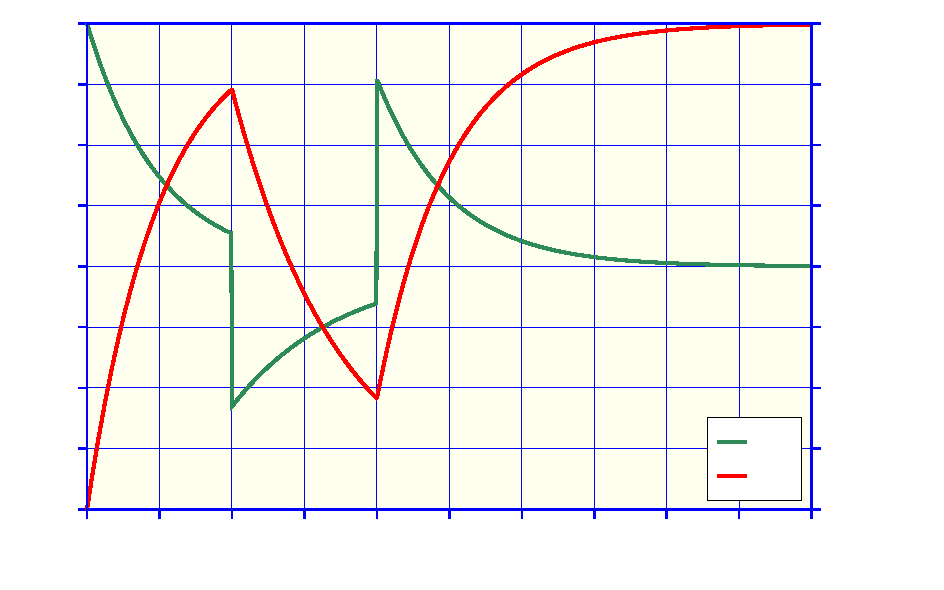
\includegraphics{Cap-Fonaments-RL-Carrega-Descarrega}}%
    \gplfronttext
  \end{picture}%
\endgroup

    \end{center}

    Per acabar, dibuixarem la mateixa funció $i(t)$ utilitzant la calculadora \emph{HP Prime}.
    \index{HP Prime!exemples} Els passos a seguir són els següents:
    \begin{dingautolist}{'312}
        \item En primer lloc premem la tecla 
\includegraphics{HPPrime-Apps.pdf} i seleccionem l'aplicació \funsfbs{Function}.

             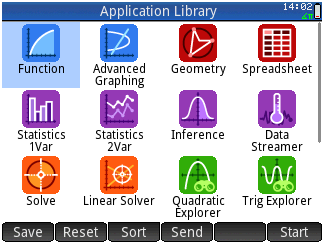
\includegraphics{Cap-Fonaments-RL-Carrega-Descarrega-HPP1.png}

        \item Tot seguit entrem en els camps \funsfbs{F1(X)}, \funsfbs{F2(X)} i \funsfbs{F3(X)} les equacions de $i_1(t)$, $i_2(t)$ i $i_3(t)$; enlloc dels valors \num{1,7293} i  \num{0,4558}, utilitzarem \funsfbs{F1(0.02)} i \funsfbs{F2(0.04)} respectivament, per tal que la calculadora els calculi automàticament. Com a variable utilitzarem \funsfbs{X} enlloc de \funsfbs{t}.

            En el camp \funsfbs{F4(X)} entrem la funció $i(t)$, amb l'ajut de la funció  \funsfbs{Heaviside(X)}. Escriurem:\break \funsfbs{F1(X) * (Heaviside(X-0)-Heaviside(X-0.02)) + F2(X) * (Heaviside(X-0.02)-Heaviside(X-0.04))\break + F3(X) * Heaviside(X-0.04)}.

            Finalment, deixem marcat el camp \funsfbs{F4(X)} i desmarquem els camps \funsfbs{F1(X)}, \funsfbs{F2(X)} i \funsfbs{F3(X)}.

            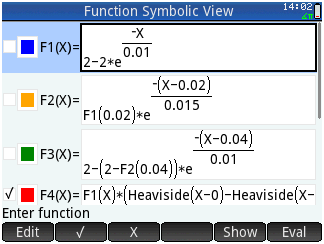
\includegraphics{Cap-Fonaments-RL-Carrega-Descarrega-HPP2.png}

            Una altra manera de crear el camp \funsfbs{F4(X)}, és usant la funció \funsfbs{IFTE(Cond,ST,SF)}; aquesta funció avalua l'expressió \funsfbs{Cond}, si el resultat   és cert executa \funsfbs{ST} i si és fals executa \funsfbs{SF}. Podem escriure per tant: \funsfbs{IFTE(X<0.02,F1(X),IFTE(X<0.04,F2(X),F3(X)))}.

            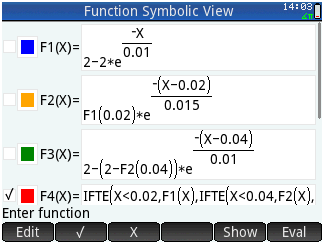
\includegraphics{Cap-Fonaments-RL-Carrega-Descarrega-HPP3.png}

        \item Ara ja podem dibuixar la funció $i(t)$.

            Comencem ajustant els paràmetres de la gràfica, prement les tecles 
\includegraphics{HPPrime-Shift.pdf} 
\includegraphics{HPPrime-Plot.pdf}; fixem els dos valors de \funsfbs{X Rng} a \funsfbs{0} i \funsfbs{0.1} respectivament, els dos valors de \funsfbs{Y Rng} a \funsfbs{0} i \funsfbs{2} respectivament, el valor de \funsfbs{X Tick} a \funsfbs{0.01}, i el valor de \funsfbs{Y Tick} a \funsfbs{0.25}.

            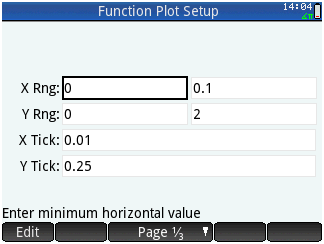
\includegraphics{Cap-Fonaments-RL-Carrega-Descarrega-HPP4.png}

        \item A continuació premem la tecla 
\includegraphics{HPPrime-Plot.pdf} i la calculadora dibuixa la gràfica.

            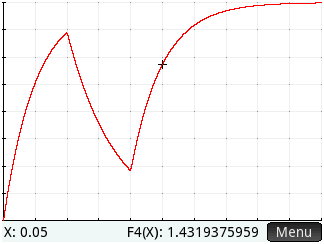
\includegraphics{Cap-Fonaments-RL-Carrega-Descarrega-HPP5.png}
    \end{dingautolist}
\end{exemple}


\subsection {Circuit R-L -- Curtcircuit en corrent altern}\index{circuit R-L!curtcircuit en corrent altern}\label{sec:ccRL}

Comencem resolent analíticament el circuit R-L de la figura \vref{pic:RL_serie_curtcircuit}, sotmès a un curtcircuit en tancar l'interruptor a l'instant $t=0$, amb la condició inicial: $i(0) = 0$; $u(t)$ és una tensió sinusoïdal, on $U$ és el seu valor eficaç, $\omega = 2 \piup f$, i $\phi$ és l'angle inicial.

Aquest circuit pot representar directament un circuit monofàsic on s'hi produeix un curtcircuit, però també pot representar en el cas d'un curtcircuit trifàsic,  el circuit equivalent per fase d'una xarxa trifàsica, on $R$ i $L$ és la impedància equivalent de la xarxa, vista des del punt del curtcircuit, i $u(t)$ és la tensió en el punt de curtcircuit en l'instant previ al curtcircuit; $u(t)$,  $R$ i $L$ representen en aquest cas, el circuit equivalent Thévenin de la xarxa en el punt del curtcircuit.

\begin{center}
    \input{Imatges/Cap-Fonaments-RL-Serie-Curtcircuit.pdf_tex}
    \captionof{figure}{Circuit R-L -- Curtcircuit en corrent altern}
    \label{pic:RL_serie_curtcircuit}
\end{center}

L'equació diferencial que lliga les variables d'aquest circuit és:
\begin{equation}
    u(t) = R i(t) + L \deriv{i(t)}{t}
\end{equation}

Resolent aquesta equació diferencial amb el valor inicial $i(0)=0$, trobem que el corrent de curtcircuit $i(t)$  que es produeix  és:
\begin{equation}
    i(t) = i\ped{ac}(t) + i\ped{dc}(t)
    \label{eq:RL_serie_curtcircuit_icc}
\end{equation}

Amb:
\begin{subequations}
\begin{align}
    i\ped{ac}(t) &= \sqrt{2} I \sin\left(\omega t + \phi - \arctan\frac{\omega L}{R}\right) \label{eq:RL_serie_curtcircuit_iac}\\[3mm]
    i\ped{dc}(t) &= -\,\sqrt{2} I\sin\left(\phi - \arctan\frac{\omega L}{R}\right) \eu^{-t R/L}\label{eq:RL_serie_curtcircuit_idc}
\end{align}
\end{subequations}

On $I$ és el valor eficaç de $i\ped{ac}(t)$; aquest valor també s'anomena valor eficaç simètric $I\ped{sim}$, i val:
\begin{equation}
    I = I\ped{sim} =\frac{U}{\sqrt{R^2+(\omega L)^2}}
    \label{eq:RL_serie_curtcircuit_I}
\end{equation}

La component $i\ped{dc}(t)$ decreix amb el pas del temps fins a fer-se zero, i finalment només queda la component $i\ped{ac}(t)$. El valor màxim de $i(t)$, anomenat valor de pic asimètric $\hat{I}\ped{asim}$, es dóna a prop de l'inici ($t\approx 0$), i depèn del valor que pren $i\ped{dc}(0)$, i per tant depèn del valor de $\sin\left(\phi - \arctan\frac{\omega L}{R}\right)$, que apareix en l'equació \eqref{eq:RL_serie_curtcircuit_idc}. En circuits força inductius ($\omega L\gg R$), $\hat{I}\ped{asim}$ és màxim per a $\phi \approx 0$, i pren el valor teòric:
\begin{equation}
    \hat{I}\ped{asim} = i\ped{dc}(0) + \sqrt{2} I\ped{sim} \approx \sqrt{2} I\ped{sim} +\sqrt{2} I\ped{sim} =2 \sqrt{2} I\ped{sim}    \label{eq:I_asim_pic}
\end{equation}


En aquest mateix cas, també és màxim el valor eficaç inicial de $i(t)$, anomenat valor eficaç asimètric $I\ped{asim}$,  i pren el valor teòric:
\begin{equation}
    I\ped{asim} = \sqrt{i\ped{dc}^2(0) + I\ped{sim}^2} \approx \sqrt{\left(\sqrt{2}I\ped{sim}\right)^2 + I\ped{sim}^2} = \sqrt{3} I\ped{sim} \label{eq:I_asim_eff}
\end{equation}

Finalment, en aquest mateix cas la relació entre $\hat{I}\ped{asim}$ i $I\ped{asim}$,   pren el valor teòric:
\begin{equation}
    \hat{I}\ped{asim} = \frac{2\sqrt{2}}{\sqrt{3}} I\ped{asim} \approx
    \num{1,633} I\ped{asim}
    %\aprox
\end{equation}

Pel mateix raonament anterior, el valor mínim de $i(t)$ en circuits força inductius, s'aconsegueix quan $\phi \approx \pm\frac{\pi}{2}$. En Aquest cas $i\ped{dc}(t)$ es fa zero des de l'inici, i només queda la component alterna $i\ped{ac}(t)$.

\begin{exemple}[Curtcircuit en un circuit R-L]\label{ex:cc-RL}
    Es tracta de calcular el corrent de curtcircuit que circula pel circuit de la Figura \vref{pic:RL_serie_curtcircuit}, amb els valors següents: $U=\SI{400}{V}, f=\SI{50}{Hz}, \phi=\SI{0}{rad}, R=\SI{9e-4}{\ohm}, L=\SI{5e-5}{H}$.

    Primer calculem els valors:
    \begin{align*}
        \omega &= 2\pi f = 2\times\pi\times\SI{50}{Hz} = \SI{314,1593}{rad/s} \\[3mm]
        \arctan\frac{\omega L}{R} &= \arctan\frac{\SI{314,1593}{rad/s}\times\SI{5e-5}{H}}{\SI{9e-4}{\ohm}} =
        \SI{1,5136}{rad}\\[3mm]
        \sin\left(\phi - \arctan\frac{\omega L}{R}\right) &= \sin(\SI{0}{rad} - \SI{1,5136}{rad})= \num{-0,9984}
    \end{align*}


    A continuació, utilitzant l'equació \eqref{eq:RL_serie_curtcircuit_I}, tenim:
    \[
        I= I\ped{sim} =\frac{\SI{400}{V}}{\sqrt{\left(\SI{9e-4}{\ohm}\right)^2+\left(\SI{314,1593}{rad/s}\times \SI{5e-5}{H}\right)^2}} =
        \SI{25423,0955}{A}
    \]

      A partir d'aquests valors i de les equacions \eqref{eq:RL_serie_curtcircuit_icc}, \eqref{eq:RL_serie_curtcircuit_iac} i \eqref{eq:RL_serie_curtcircuit_idc}, tenim:
    \begin{align*}
        i\ped{ac}(t) &= \num{35953,6865}\sin(\num{314,1593}\,t-\num{1,5136}) \\[0.3cm]
        i\ped{dc}(t) &= \num{35894,8169}\,\eu^{-18 t}\\[0.3cm]
        i(t) &= \num{35953,6865}\sin(\num{314,1593}\,t-\num{1,5136}) + \num{35894,8169}\,\eu^{-18 t}
    \end{align*}

    Finalment, donat que es compleix $\phi=0$ i $\omega L \,(\SI{157,2e-4}{\ohm}) \gg R\, (\SI{9e-4}{\ohm}) $, podem utilitzar les equacions \eqref{eq:I_asim_pic} i \eqref{eq:I_asim_eff}:
    \begin{align*}
        \hat{I}\ped{asim} &= 2 \sqrt{2} I\ped{sim}= 2 \times \sqrt{2} \times \SI{25423,0955}{A} = \SI{71,9}{kA}\\[0.3cm]
        I\ped{asim} &= \sqrt{3} I\ped{sim}= \sqrt{3} \times \SI{25423,0955}{A} = \SI{44,0}{kA}
    \end{align*}

    Per acabar, representem les funcions $i\ped{dc}(t)$, $i\ped{ac}(t)$ i $i(t)$:
    \begin{center}
        % GNUPLOT: LaTeX picture with Postscript
\begingroup
  \makeatletter
  \providecommand\color[2][]{%
    \GenericError{(gnuplot) \space\space\space\@spaces}{%
      Package color not loaded in conjunction with
      terminal option `colourtext'%
    }{See the gnuplot documentation for explanation.%
    }{Either use 'blacktext' in gnuplot or load the package
      color.sty in LaTeX.}%
    \renewcommand\color[2][]{}%
  }%
  \providecommand\includegraphics[2][]{%
    \GenericError{(gnuplot) \space\space\space\@spaces}{%
      Package graphicx or graphics not loaded%
    }{See the gnuplot documentation for explanation.%
    }{The gnuplot epslatex terminal needs graphicx.sty or graphics.sty.}%
    \renewcommand\includegraphics[2][]{}%
  }%
  \providecommand\rotatebox[2]{#2}%
  \@ifundefined{ifGPcolor}{%
    \newif\ifGPcolor
    \GPcolortrue
  }{}%
  \@ifundefined{ifGPblacktext}{%
    \newif\ifGPblacktext
    \GPblacktexttrue
  }{}%
  % define a \g@addto@macro without @ in the name:
  \let\gplgaddtomacro\g@addto@macro
  % define empty templates for all commands taking text:
  \gdef\gplbacktext{}%
  \gdef\gplfronttext{}%
  \makeatother
  \ifGPblacktext
    % no textcolor at all
    \def\colorrgb#1{}%
    \def\colorgray#1{}%
  \else
    % gray or color?
    \ifGPcolor
      \def\colorrgb#1{\color[rgb]{#1}}%
      \def\colorgray#1{\color[gray]{#1}}%
      \expandafter\def\csname LTw\endcsname{\color{white}}%
      \expandafter\def\csname LTb\endcsname{\color{black}}%
      \expandafter\def\csname LTa\endcsname{\color{black}}%
      \expandafter\def\csname LT0\endcsname{\color[rgb]{1,0,0}}%
      \expandafter\def\csname LT1\endcsname{\color[rgb]{0,1,0}}%
      \expandafter\def\csname LT2\endcsname{\color[rgb]{0,0,1}}%
      \expandafter\def\csname LT3\endcsname{\color[rgb]{1,0,1}}%
      \expandafter\def\csname LT4\endcsname{\color[rgb]{0,1,1}}%
      \expandafter\def\csname LT5\endcsname{\color[rgb]{1,1,0}}%
      \expandafter\def\csname LT6\endcsname{\color[rgb]{0,0,0}}%
      \expandafter\def\csname LT7\endcsname{\color[rgb]{1,0.3,0}}%
      \expandafter\def\csname LT8\endcsname{\color[rgb]{0.5,0.5,0.5}}%
    \else
      % gray
      \def\colorrgb#1{\color{black}}%
      \def\colorgray#1{\color[gray]{#1}}%
      \expandafter\def\csname LTw\endcsname{\color{white}}%
      \expandafter\def\csname LTb\endcsname{\color{black}}%
      \expandafter\def\csname LTa\endcsname{\color{black}}%
      \expandafter\def\csname LT0\endcsname{\color{black}}%
      \expandafter\def\csname LT1\endcsname{\color{black}}%
      \expandafter\def\csname LT2\endcsname{\color{black}}%
      \expandafter\def\csname LT3\endcsname{\color{black}}%
      \expandafter\def\csname LT4\endcsname{\color{black}}%
      \expandafter\def\csname LT5\endcsname{\color{black}}%
      \expandafter\def\csname LT6\endcsname{\color{black}}%
      \expandafter\def\csname LT7\endcsname{\color{black}}%
      \expandafter\def\csname LT8\endcsname{\color{black}}%
    \fi
  \fi
    \setlength{\unitlength}{0.0500bp}%
    \ifx\gptboxheight\undefined%
      \newlength{\gptboxheight}%
      \newlength{\gptboxwidth}%
      \newsavebox{\gptboxtext}%
    \fi%
    \setlength{\fboxrule}{0.5pt}%
    \setlength{\fboxsep}{1pt}%
\begin{picture}(8220.00,4800.00)%
    \gplgaddtomacro\gplbacktext{%
      \colorrgb{0.00,0.00,0.00}%%
      \put(655,787){\makebox(0,0)[r]{\strut{}-40}}%
      \colorrgb{0.00,0.00,0.00}%%
      \put(655,1419){\makebox(0,0)[r]{\strut{}-20}}%
      \colorrgb{0.00,0.00,0.00}%%
      \put(655,2051){\makebox(0,0)[r]{\strut{} 0}}%
      \colorrgb{0.00,0.00,0.00}%%
      \put(655,2684){\makebox(0,0)[r]{\strut{} 20}}%
      \colorrgb{0.00,0.00,0.00}%%
      \put(655,3316){\makebox(0,0)[r]{\strut{} 40}}%
      \colorrgb{0.00,0.00,0.00}%%
      \put(655,3948){\makebox(0,0)[r]{\strut{} 60}}%
      \colorrgb{0.00,0.00,0.00}%%
      \put(655,4580){\makebox(0,0)[r]{\strut{} 80}}%
      \colorrgb{0.00,0.00,0.00}%%
      \put(839,481){\makebox(0,0){\strut{}$0$}}%
      \colorrgb{0.00,0.00,0.00}%%
      \put(1537,481){\makebox(0,0){\strut{}$20$}}%
      \colorrgb{0.00,0.00,0.00}%%
      \put(2235,481){\makebox(0,0){\strut{}$40$}}%
      \colorrgb{0.00,0.00,0.00}%%
      \put(2933,481){\makebox(0,0){\strut{}$60$}}%
      \colorrgb{0.00,0.00,0.00}%%
      \put(3631,481){\makebox(0,0){\strut{}$80$}}%
      \colorrgb{0.00,0.00,0.00}%%
      \put(4329,481){\makebox(0,0){\strut{}$100$}}%
      \colorrgb{0.00,0.00,0.00}%%
      \put(5027,481){\makebox(0,0){\strut{}$120$}}%
      \colorrgb{0.00,0.00,0.00}%%
      \put(5725,481){\makebox(0,0){\strut{}$140$}}%
      \colorrgb{0.00,0.00,0.00}%%
      \put(6423,481){\makebox(0,0){\strut{}$160$}}%
      \colorrgb{0.00,0.00,0.00}%%
      \put(7121,481){\makebox(0,0){\strut{}$180$}}%
      \colorrgb{0.00,0.00,0.00}%%
      \put(7819,481){\makebox(0,0){\strut{}$200$}}%
    }%
    \gplgaddtomacro\gplfronttext{%
      \csname LTb\endcsname%%
      \put(158,2683){\rotatebox{-270}{\makebox(0,0){\strut{}$i\ped{dc}(t)\, / \,\unit{kA}, \quad i\ped{ac}(t)\, / \,\unit{kA}, \quad i(t)\, / \,\unit{kA}$}}}%
      \csname LTb\endcsname%%
      \put(7873,2683){\rotatebox{-270}{\makebox(0,0){\strut{}}}}%
      \csname LTb\endcsname%%
      \put(4329,153){\makebox(0,0){\strut{}$t\, / \,\unit{ms}$}}%
      \csname LTb\endcsname%%
      \put(4329,4471){\makebox(0,0){\strut{}}}%
      \csname LTb\endcsname%%
      \put(4329,4580){\makebox(0,0){\strut{}}}%
      \csname LTb\endcsname%%
      \put(7145,4329){\makebox(0,0){\strut{}}}%
      \csname LTb\endcsname%%
      \put(7043,4247){\makebox(0,0)[l]{\strut{}$i\ped{dc}(t)$}}%
      \csname LTb\endcsname%%
      \put(7043,3919){\makebox(0,0)[l]{\strut{}$i\ped{ac}(t)$}}%
      \csname LTb\endcsname%%
      \put(7043,3591){\makebox(0,0)[l]{\strut{}$i(t)$}}%
    }%
    \gplbacktext
    \put(0,0){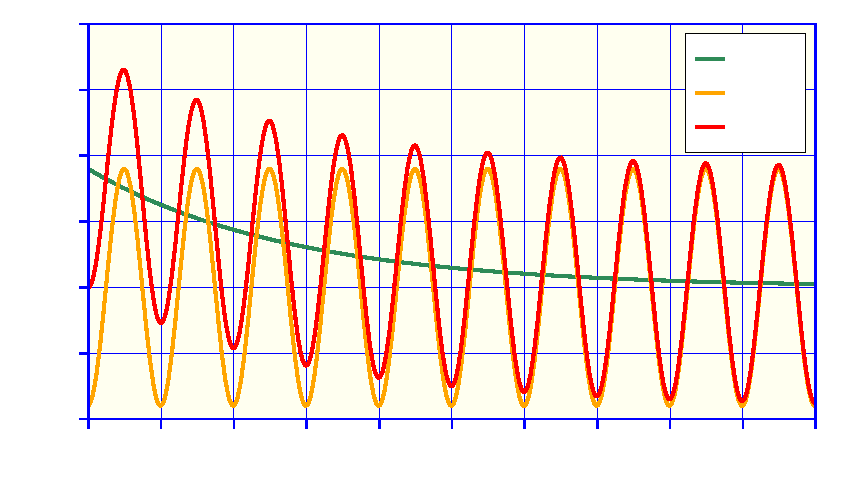
\includegraphics{Cap-Fonaments-RL-Serie-Curtcircuit-Exemple}}%
    \gplfronttext
  \end{picture}%
\endgroup

    \end{center}
\end{exemple}


Tal com s'ha dit anteriorment, el valor de $\hat{I}\ped{asim}$ donat per l'equació \eqref{eq:I_asim_pic}, en el cas de $\phi \approx 0$ i $\omega L\gg R$, és teòric. La norma CEI 60909-1 dóna valors més exactes per a $\hat{I}\ped{asim}$, en el cas de $\phi \approx 0$, segons l'expressió següent:\index{CEI!60909-1}
\begin{equation}
    \hat{I}\ped{asim} = \kappa \sqrt{2} I\ped{sim} \label{eq:I_asim_CEI}
\end{equation}

On el factor $\kappa$ ve donat per l'expressió:
\begin{equation}
    \kappa = 1{,}02 + 0{,}98 \,\eu^{-3\frac{R}{\omega L}}\label{eq:kappa_CEI}
\end{equation}

Quan es compleix $\omega L\gg R$, tenim $\kappa \approx 2$, i l'equació \eqref{eq:I_asim_CEI} dóna el mateix valor que l'equació \eqref{eq:I_asim_pic}.

En el cas de la xarxa de l'apartat anterior, la relació $\frac{R}{\omega L}$ és fàcil de  calcular, no obstant, en xarxes grans on hi ha moltes branques, els valors de $\frac{R}{\omega L}$ de cadascuna de les branques no coincideix en general amb el valor calculat en el punt del curtcircuit, utilitzant els valors $R$ i $\omega L$ de la xarxa equivalent en aquest punt. La mateixa norma CEI 60909-1 explica com cal procedir en aquests casos.


\begin{exemple}[Corrent de pic asimètric]\label{ex:corrent-pic}
    Es tracta de calcular el corrent de pic asimètric del corrent de curtcircuit de l'exemple \ref{ex:cc-RL} segons la norma CEI 60909-1.

    El valor de curtcircuit eficaç simètric calculat a l'exemple \vref{ex:cc-RL} és: $I\ped{sim}= \SI{25,4}{kA}$.

    Primer calculem $\kappa$ utilitzant l'equació \eqref{eq:kappa_CEI}:
    \[
    \kappa = \num{1,02} + \num{0,98} \,\eu^{-3\frac{\SI{9e-4}{\ohm}}{\SI{314,1593}{rad/s}\, \times\, \SI{5e-5}{H}}} = \num{1,8452}
    \]

    I a continuació calculem $\hat{I}\ped{asim}$ utilitzant l'equació \eqref{eq:I_asim_CEI}:
    \[
    \hat{I}\ped{asim} = \num{1,8452} \times \sqrt{2} \times \SI{25,4}{kA} = \SI{66,3}{kA}
    \]

    Aquest valor és més a prop del real, tal com es pot veure en la gràfica de l'exemple  \ref{ex:cc-RL}, que el valor de  \SI{71,9}{kA} obtingut en aquell exemple.

    Trobarem a continuació el valor exacte  del corrent de pic utilitzant la calculadora  \emph{HP Prime}.
    \index{HP Prime!exemples} Els passos a seguir són els següents:

     \begin{dingautolist}{'312}

        \item En primer lloc premem la tecla 
\includegraphics{HPPrime-Apps.pdf} i seleccionem l'aplicació \funsfbs{Function}.

             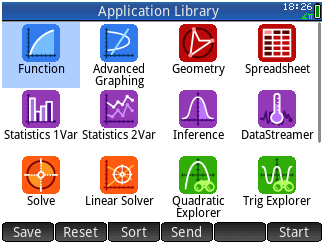
\includegraphics{Cap-Fonaments-RL-Serie-Curtcircuit-HPP1.png}

        \item Tot seguit entrem en els camps \funsfbs{F1(X)} i \funsfbs{F2(X)} les equacions de $i\ped{ac}(t)$ i $i\ped{dc}(t)$ que hem calculat en l'exemple \vref{ex:cc-RL}; com a variable utilitzarem \funsfbs{X} enlloc de \funsfbs{t}.

            En el camp \funsfbs{F3(X)} entrem \funsfbs{F1(X)+F2(X)}.

            Finalment, deixem marcat el camp \funsfbs{F3(X)} i desmarquem els camps \funsfbs{F1(X)} i \funsfbs{F2(X)}. D'aquesta manera la calculadora només dibuixarà la funció total $i(t)$, i no les parcials $i\ped{ac}(t)$ i $i\ped{dc}(t)$.


            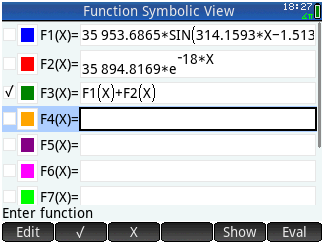
\includegraphics{Cap-Fonaments-RL-Serie-Curtcircuit-HPP2.png}

        \item Ara ja podem dibuixar la funció del corrent total de curtcircuit.

            Comencem ajustant els paràmetres de la gràfica, prement les tecles 
\includegraphics{HPPrime-Shift.pdf} 
\includegraphics{HPPrime-Plot.pdf}; fixem els dos valors de \funsfbs{X Rng} a \funsfbs{0} i \funsfbs{0.1} respectivament, els dos valors de \funsfbs{Y Rng} a \funsfbs{-40000} i \funsfbs{80000} respectivament, el valor de \funsfbs{X Tick} a \funsfbs{0.01}, i el valor de \funsfbs{Y Tick} a \funsfbs{10000}.

            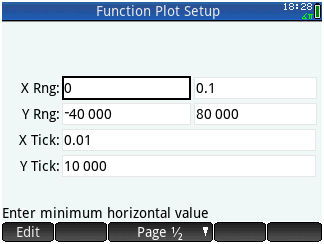
\includegraphics{Cap-Fonaments-RL-Serie-Curtcircuit-HPP3.png}

        \item A continuació premem la tecla 
\includegraphics{HPPrime-Plot.pdf} i la calculadora dibuixa la gràfica; cal verificar prèviament que la calculadora estigui en el mode angular radiants, ja que en cas contrari el dibuix que obtindríem no seria correcte. El cursor queda situat automàticament al centre de la pantalla.

            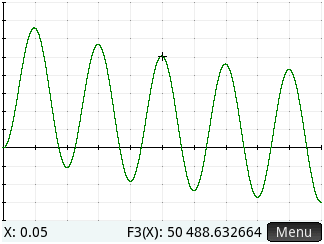
\includegraphics{Cap-Fonaments-RL-Serie-Curtcircuit-HPP4.png}

        \item Premem ara el botó \hpbutton{Menu}, i a continuació situem el cursor amb el dit a prop del primer màxim de la funció.

            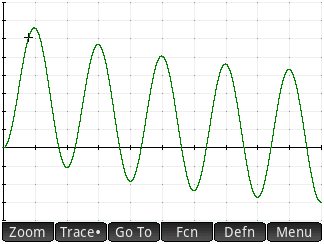
\includegraphics{Cap-Fonaments-RL-Serie-Curtcircuit-HPP5.png}

        \item Premem a continuació el botó \hpbutton{\phantom{x}Fcn\phantom{x}} i seleccionem la funció \funsfbs{Extremum} del menú que apareix.

            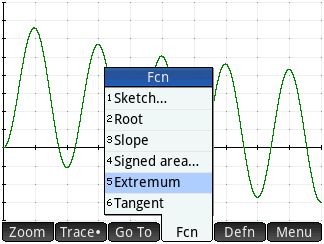
\includegraphics{Cap-Fonaments-RL-Serie-Curtcircuit-HPP6.png}

        \item La calculadora ens dóna immediatament el valor del punt màxim de la funció, a la part inferior de la pantalla.

            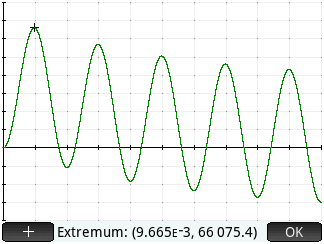
\includegraphics{Cap-Fonaments-RL-Serie-Curtcircuit-HPP7.png}

            El pic es troba doncs a: $t=\SI{9,6649}{ms}$, i té el valor:  $\hat{I}\ped{asim}=\SI{66075,4}{A}$.
    \end{dingautolist}

\end{exemple}


\section{Resolució de xarxes mitjançant el mètode de les malles}\label{sec:metode-malles}
\index{metode@mètode de les malles}

En el capítol \ref{chap:nusos} es presenta un mètode general per resoldre xarxes elèctriques, que tot i que es pot fer servir per a xarxes de qualsevol dimensió, és més normal utilitzar-lo en xarxes on el nombre de nusos és elevat.

Es presenta a continuació el mètode de les malles, que és l'utilitzat més usualment alhora de resoldre xarxes de pocs nusos; té l'avantatja respecte d'altres mètodes de reduir el nombre d'equacions a resoldre. Utilitzarem com a exemple la xarxa de la figura \vref{pic:metode_malles}:

\begin{center}
    \input{Imatges/Cap-CalcBas-Malles.pdf_tex}
    \captionof{figure}{Mètode de les malles} \label{pic:metode_malles}
\end{center}

En aquesta xarxa, les dues fonts de tensió $\cmplx{E}_1$ i $\cmplx{E}_2$ i les sis impedàncies $\cmplx{Z}_1$, $\cmplx{Z}_2$, $\cmplx{Z}_3$, $\cmplx{Z}_4$, $\cmplx{Z}_5$ i $\cmplx{Z}_6$  són valors coneguts, i les incògnites són els sis corrents $\cmplx{I}_1$, $\cmplx{I}_2$, $\cmplx{I}_3$, $\cmplx{I}_4$, $\cmplx{I}_5$ i $\cmplx{I}_6$.

El mètode tradicional utilitzat per resoldre aquesta xarxa, consisteix en crear un sistema  de sis equacions lineals amb sis incògnites (les intensitats), utilitzant  la 1a i 2a lleis de Kirchhoff, i resoldre'l.

El mètode de les malles utilitza uns corrents ficticis de malla, $\cmplx{I}\ped{M_1}$, $\cmplx{I}\ped{M_2}$ i $\cmplx{I}\ped{M_3}$, que ens permeten reduir el nombre d'equacions lineals del  sistema que haurem de resoldre.



En primer lloc cal definir què entenem per una malla: una malla és un camí tancat que no conté dins seu cap altre camí tancat. En aquest sentit tenim en la xarxa de la figura \vref{pic:metode_malles} tres malles: $\cmplx{Z}_1$--$\cmplx{Z}_3$--$\cmplx{E}_1$, $\cmplx{Z}_2$--$\cmplx{Z}_5$--$\cmplx{Z}_4$--$\cmplx{Z}_3$ i $\cmplx{Z}_5$--$\cmplx{Z}_6$--$\cmplx{E}_2$.

Les relacions entre els corrents de cadascuna de les branques de la xarxa i els corrents de malla són:
\begin{subequations}
\begin{align}
    \cmplx{I}_1 &= \cmplx{I}\ped{M_1} \label{eq:malles1} \\[0.5ex]
    \cmplx{I}_2 &= -\cmplx{I}\ped{M_2} \\[0.5ex]
    \cmplx{I}_3 &= \cmplx{I}\ped{M_1}-\cmplx{I}\ped{M_2} \\[0.5ex]
    \cmplx{I}_4 &= \cmplx{I}\ped{M_2} \\[0.5ex]
    \cmplx{I}_5 &= \cmplx{I}\ped{M_2}-\cmplx{I}\ped{M_3} \\[0.5ex]
    \cmplx{I}_6 &= -\cmplx{I}\ped{M_3} \label{eq:malles2}
\end{align}
\end{subequations}

Per resoldre la xarxa de la figura \vref{pic:metode_malles}, hem de plantejar la 2a llei de Kirchhoff per a cadascuna de les tres malles; això ens proporcionarà el següent sistema d'equacions lineals de tres equacions amb tres incògnites ($\cmplx{I}\ped{M_1}$, $\cmplx{I}\ped{M_2}$ i $\cmplx{I}\ped{M_3}$):
\begin{subequations}
\begin{align}
    \cmplx{E}_1 &= \cmplx{Z}_1 \cmplx{I}\ped{M_1} + \cmplx{Z}_3 (\cmplx{I}\ped{M_1}-\cmplx{I}\ped{M_2}) \\[0.5ex]
    0 &= \cmplx{Z}_2 \cmplx{I}\ped{M_2} + \cmplx{Z}_5(\cmplx{I}\ped{M_2}-\cmplx{I}\ped{M_3}) + \cmplx{Z}_4 \cmplx{I}\ped{M_2} + \cmplx{Z}_3(\cmplx{I}\ped{M_2}-\cmplx{I}\ped{M_1}) \\[0.5ex]
    -\cmplx{E}_2 &=  \cmplx{Z}_5 (\cmplx{I}\ped{M_3}-\cmplx{I}\ped{M_2})+\cmplx{Z}_6 \cmplx{I}\ped{M_3}
\end{align}
\end{subequations}

Agrupant termes tenim:
\begin{subequations}
\begin{align}
    (\cmplx{Z}_1 + \cmplx{Z}_3) \cmplx{I}\ped{M_1} - \cmplx{Z}_3 \cmplx{I}\ped{M_2} &= \cmplx{E}_1 \\[0.5ex]
    -\cmplx{Z}_3 \cmplx{I}\ped{M_1} + (\cmplx{Z}_2 + \cmplx{Z}_3+ \cmplx{Z}_4+ \cmplx{Z}_5)\cmplx{I}\ped{M_2} - \cmplx{Z}_5 \cmplx{I}\ped{M_3} &= 0 \\[0.5ex]
     -\cmplx{Z}_5 \cmplx{I}\ped{M_2} +  (\cmplx{Z}_5 + \cmplx{Z}_6) \cmplx{I}\ped{M_3} &= -\cmplx{E}_2
\end{align}
\end{subequations}

O en forma matricial:
\begin{equation}\label{eq:malles-mat}
  \left(
    \begin{array}{ccc}
      \cmplx{Z}_1 + \cmplx{Z}_3 & -\cmplx{Z}_3 & 0 \\
      -\cmplx{Z}_3 & \cmplx{Z}_2 + \cmplx{Z}_3+ \cmplx{Z}_4+ \cmplx{Z}_5 & -\cmplx{Z}_5 \\
      0 & -\cmplx{Z}_5 & \cmplx{Z}_5 + \cmplx{Z}_6 \\
    \end{array}
  \right)
  \cdot
  \left(
      \begin{array}{c}
        \cmplx{I}\ped{M_1} \\
        \cmplx{I}\ped{M_2} \\
        \cmplx{I}\ped{M_3} \\
      \end{array}
  \right)
  =
  \left(
      \begin{array}{c}
        \cmplx{E}_1 \\
        0 \\
        -\cmplx{E}_2 \\
      \end{array}
  \right)
\end{equation}

El que queda ara per fer és resoldre aquest sistema d'equacions lineals per tal de trobar $\cmplx{I}\ped{M_1}$, $\cmplx{I}\ped{M_2}$ i $\cmplx{I}\ped{M_3}$, i a continuació utilitzar les equacions \eqref{eq:malles1} a \eqref{eq:malles2} per trobar les intensitats de cadascuna de les branques.


L'equació \eqref{eq:malles-mat} pot escriure's de forma general com:
\begin{equation}
  \mcmplx{Z} \mcmplx{I}\ped{M} = \mcmplx{E}
\end{equation}

On  $\mcmplx{Z}$ és la matriu d'impedàncies, $\mcmplx{E}$ és el vector de fonts de tensió, i $\mcmplx{I}\ped{M}$ és el vector de les intensitats de malla. Quan no hi ha acoblaments magnètics entre branques, la matriu d'impedàncies $\mcmplx{Z}$ i el vector de fonts de tensió $\mcmplx{E}$ poden formar-se de manera directa seguint els passos següents:
\begin{dingautolist}{'312}
   \item S'assigna a cada malla un número començant per l'1.

          En el nostre exemple les malles s'han numerat 1, 2 i 3, d'esquerra a dreta.
   \item Es dibuixa per a  cada malla el seu corrent de malla, tenint en compte que tots tinguin el mateix sentit de gir.

       En el nostre exemple tots els corrents giren en sentit horari.
   \item Cada element de la diagonal de la matriu d'impedàncies és igual a la suma de les impedàncies que formen cada malla.

       En el nostre exemple tenim: $\mcmplx{Z}(1,1)=\cmplx{Z}_1 + \cmplx{Z}_3$, $\mcmplx{Z}(2,2)=\cmplx{Z}_2 + \cmplx{Z}_3+ \cmplx{Z}_4+ \cmplx{Z}_5$, i $\mcmplx{Z}(3,3)=\cmplx{Z}_5 + \cmplx{Z}_6$.
   \item Cada element de fora de la diagonal de la matriu d'impedàncies és igual a la suma canviada de signe de les impedàncies en comú a les dues malles corresponents.

        En el nostre exemple les malles 1 i 2 tenen $\cmplx{Z}_3$ com a impedància en comú, i per tant tenim: $\mcmplx{Z}(1,2)=\mcmplx{Z}(2,1)= -\cmplx{Z}_3$, les malles 2 i 3 tenen $\cmplx{Z}_5$ com a impedància en comú, i per tant  tenim: $\mcmplx{Z}(2,3)=\mcmplx{Z}(3,2)= -\cmplx{Z}_5$, i les malles 1 i 3 no tenen cap impedància en comú, i per tant  tenim: $\mcmplx{Z}(1,3)=\mcmplx{Z}(3,1)= 0$.
    \item Cada element del vector de fonts de tensió és igual a la suma de les fonts de tensió que formen part de cada malla; la contribució a la suma de cada font de tensió serà positiva o negativa, segons que la seva força electromotriu tingui el mateix sentit que el corrent de malla, o que que tingui el sentit contrari.

         En el nostre exemple $\cmplx{E}_1$ i $\cmplx{I}\ped{M1}$ tenen el mateix sentit, i per tant tenim:   $\mcmplx{E}(1) = \cmplx{E}_1$, en canvi $\cmplx{E}_2$ i $\cmplx{I}\ped{M3}$ tenen   sentits contraris, i per tant   tenim:   $\mcmplx{E}(3) = -\cmplx{E}_2$, i donat que la malla 2 no té cap font de tensió  tenim:   $\mcmplx{E}(2) = 0$.
\end{dingautolist}

\begin{exemple}[Aplicació del mètode de les malles]\label{ex:malles}
    Es tracta de trobar els sis corrents de la xarxa de la figura \vref{pic:metode_malles}, amb els valors numèrics: $\cmplx{E}_1=\SI{5}{V}$, $\cmplx{E}_2=\SI{2}{V}$, $\cmplx{Z}_1=\cmplx{Z}_2=\cmplx{Z}_3=\cmplx{Z}_4=\cmplx{Z}_5=\cmplx{Z}_6=\SI{1}{\ohm}$.

    Donat que tots els valor són reals, prescindirem de la notació complexa. Posant valors numèrics a l'equació \eqref{eq:malles-mat}, tenim:

    \[
      \left(
        \begin{array}{ccc}
          2 & -1 &  0 \\
         -1 &  4 & -1 \\
          0 &  -1 & 2 \\
        \end{array}
      \right)
      \cdot
      \left(
          \begin{array}{c}
            I\ped{M_1} \\
            I\ped{M_2} \\
            I\ped{M_3} \\
          \end{array}
      \right)
      =
      \left(
          \begin{array}{c}
            5 \\
            0 \\
            -2 \\
          \end{array}
      \right)
    \]

    Resoldrem aquest sistema d'equacions lineals utilitzant la calculadora \emph{HP Prime}.\index{HP Prime!exemples} Els passos a seguir són els següents:

    \begin{dingautolist}{'312}
     \item En primer lloc premem la tecla 
\includegraphics{HPPrime-Apps.pdf} i seleccionem l'aplicació \funsfbs{Linear Solver}.

         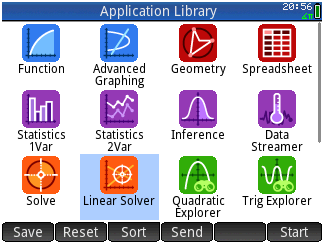
\includegraphics{Cap-CalcBas-malles-HPP1.png}
    \item A continuació només cal entrar els valors del sistema a resoldre, i la calculadora ens mostra directament la solució.

         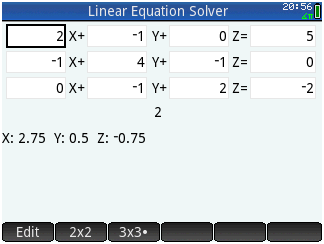
\includegraphics{Cap-CalcBas-malles-HPP2.png}
    \end{dingautolist}

    Així doncs, la solució és:
    \begin{align*}
        I\ped{M_1} &= \SI{2,75}{A} \\[0.5ex]
        I\ped{M_2} &= \SI{0,5}{A} \\[0.5ex]
        I\ped{M_3} &= \SI{-0,75}{A}
    \end{align*}

    Finalment, utilitzant les equacions \eqref{eq:malles1} a \eqref{eq:malles2} tenim:
    \begin{align*}
        I_1 &= \SI{2,75}{A} \\[0.5ex]
        I_2 &= \SI{-0,5}{A} \\[0.5ex]
        I_3 &= \SI{2,25}{A} \\[0.5ex]
        I_4 &= \SI{0,5}{A} \\[0.5ex]
        I_5 &=  \SI{1,25}{A} \\[0.5ex]
        I_6 &= \SI{0,75}{A}
    \end{align*}

\end{exemple}

